%%%%%%%%%%%%%%%%%%%%%%%%%%%%%%%%%%%%%%%%%%%%%%%%%%%%%%%%%%%%%%%%%%%%%%%%%%%%%%%%
% input_validation.tex
%%%%%%%%%%%%%%%%%%%%%%%%%%%%%%%%%%%%%%%%%%%%%%%%%%%%%%%%%%%%%%%%%%%%%%%%%%%%%%%%
\chapter{Partial Disappearance Event Classification}
\label{sec:BDT}
Unlike the total disappearance region, where rejecting standalone muons and limiting calorimeter energy is sufficient to control muon backgrounds, the partial disappearance region must separate potential signal events based on a large number of input features, often with subtle correlations between them.
The primary distinguishing feature of signal events in this region is a large mismatch in the energy of the nearest standalone muon and the selected probe track, but the requirement that the standalone muon have less than 40$\%$ of the probe track energy still leaves a large number of background events from DY muons.

Primarily caused by poorly reconstructed standalone muons, these backgrounds often have lower fit qualities, CSC hits closer to the projected track, and larger HCAL energy deposits.
These effects are not fully independent; for instance, muons with large HCAL energy may have genuine track deflection from SM scattering, so their CSC hits will be more consistent across stations resulting in better fit qualities.
Similarly, muons with low quality fits will often have several missing CSC hits, producing standalone muons with large energy differences to the real muothe real muons often have differences in $\phi$ of between the standalone muon and probe track which are correlated with the track charge, as the lower energy deflected muons are deflected more by the magnetic field.
Signal events may also have significant CSC hit displacements from the projected track location due to the angular scatter caused by \dbrem, or missing energy in several HCAL depths from muons deflecting away from the expected HE cells.

To take advantage of the wide variety of weak input separators available in this region, as well as the correlations between them, a BDT classifier is used to reduce these inputs to one classification variable.

\section{Boosted Decision Trees}
Boosted decision trees are a type of supervised machine learning where separate additive functions are used to map a set of inputs to a single output.
Each individual function consists of a single 'tree', where input data is split recursively over a series of 'depths'. 
The depths are made of 'nodes', where the data is split based on a selection applied to some input variables, and 'leaves', a terminal value of the tree where a value is output.
Each node is chosen to optimize the information gained by the split made, and the tree continues until the maximum depth is reached or no further information is gained.

The "boosting" originates from the method used to produce many input trees and combine their outputs~\cite{GradBoost}. 
As it is normally impossible to create all potential tree structures, trees are generated iteratively by starting from a single leaf and adding branches which minimize the "loss function", which is some function used to quantify the distance between the true and predicted value.
In this analysis, the loss function is chosen to be a binary logistic function,

\begin{equation}
	\label{binLogFunc}
	L = - \frac{1}{N} \sum_{i=1}^{N} y_i log(p(y_i)) + (1-y_i) log(1-p(y_i))
\end{equation} 

where N is the total number of training events, $y_i$ is the true value of each point with zero for background and one for signal, and $p(y_i)$ is the output score for that point.
The binary logistic loss function is small for predictions which are close to the true value, and increases exponentially for predictions which are far from the true value to increase the penalty for incorrect classification.

Each tree is then given a weight according to its accuracy and combined to produce a continuous output score from zero to one, with events near zero being the most background-like and events near one being the most signal-like. 
After each step of optimizing the tree weights, the training data is re-weighted to increase the importance of events that are more frequently misclassified in order to more quickly approach the strongest classification.
The tree optimization and re-weighting is then continued for several iterations in order to minimize an objective function consisting of the loss function and a regularization function, which reduces overtraining by penalizing the complexity of the trees used.

The main advantage of tree boosting is that it allows many weak classifiers in the individual trees to be combined into one strong classifier using the ensemble output score.
In this analysis, a "Gradient" BDT was used, provided by the XGBoost framework~\cite{XGBoost} interfaced with Scikit-learn~\cite{scikit}. 

The BDT is trained using only signal and DY MC, as the preselection and standalone muon requirements alone are significant enough to control the rate of $\mu+X$ events. 
An equally weighted combination of all signal masses is used for the signal sample during the BDT training.

\section{Inputs}
There are 21 event variables which are used as inputs to the BDT, which can be grouped into five categories.

The first are variables related to the probe track kinematics. 
The $p_t$, $\eta$, $\phi$, and charge of the probe track are used in order to allow the network to encode effects which may be local to certain regions of the detector.
As the CSCs have known gaps in particular depths and regions of poor reconstruction, these variables can help identify tracks which may be expected to have lower quality.

Second are the standalone muon kinematics, specifically its energy and $\chi^{2}$. %\Cref{fig:staKin}).
The $\chi^{2}$ of the standalone muon fit is used to measure the quality of its fit, and helps to separate muons with genuine energy loss from those with poor reconstruction.
The overall standalone muon energy is used in addition to the difference in standalone muon and probe track energy in case there are energy-dependent factors that may be lost when using only the relative measure.

%\begin{figure}[htpb]
%	\label{fig:staKin}
%	\includegraphics[width=0.45\textwidth]{figures/}
%	\hspace{0.01\textwidth}
%	\includegraphics[width=0.45\textwidth]{figures/}
%	\caption[short caption]{long caption}
%\end{figure}

The third category are the CSC segment distances.
In each CSC station, the minimum $\Delta$R is measured from each CSC segment to the projected probe track at its position of closest approach to that segment.
Signal events often see small displacements in these CSC hits which are consistent across stations, while background events often have very close CSC hits in every station or have several stations with no nearby segments resulting in poor fits and significant mis-measured energy.

Fourth, the difference between the standalone muon and the probe track in energy, $\Delta$R, and $\Delta \phi$ are used.
Signal events tend to have significantly lower energy standalone muons from energy loss to the \aprime, as well as larger standalone muon $\Delta$R from the angular deflection in \dbrem and additional curvature in the magnetic field.
To help distinguish angular changes caused by energy loss, the $\Delta \phi$ between the standalone muon and probe track is multiplied by the track charge, as differences due to random scatters and poor reconstruction should have no correlation with charge while deflection from real energy loss will change direction with the track charge.

Lastly, the HCAL energy in each depth along the probe trajectory is used to identify events with high energy deposits corresponding to SM processes, or multiple low energy deposits corresponding to potential signal events.
The number of depths traversed by any given muon depends on its position in HCAL.
To accomodate this, depths in HCAL which are not along the track trajectory are assigned an energy of -1 GeV. 

The distribution of the highest-performing input variable in each category for DY MC and several signal masses is shown in \Cref{fig:bdtFeatures}.

\begin{figure}[htpb]
	\centering
	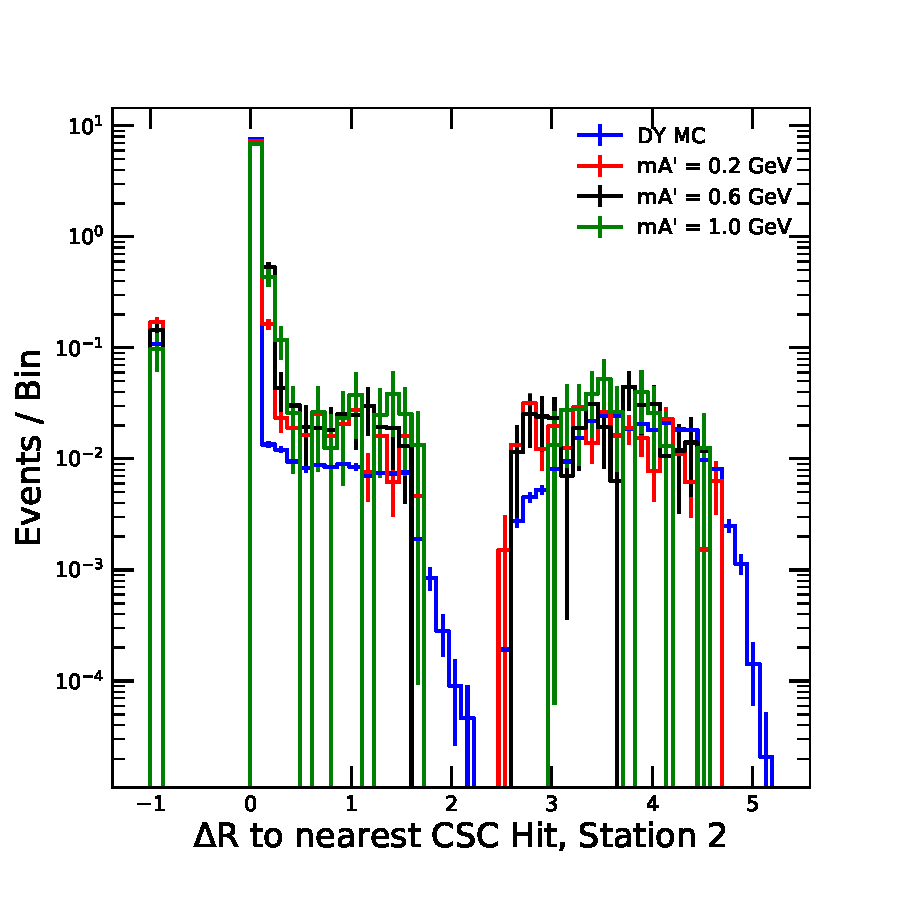
\includegraphics[width=0.45\textwidth]{figures/bdtInputFeatscscDRbyStation_1.pdf}
	\hspace{0.01\textwidth}
	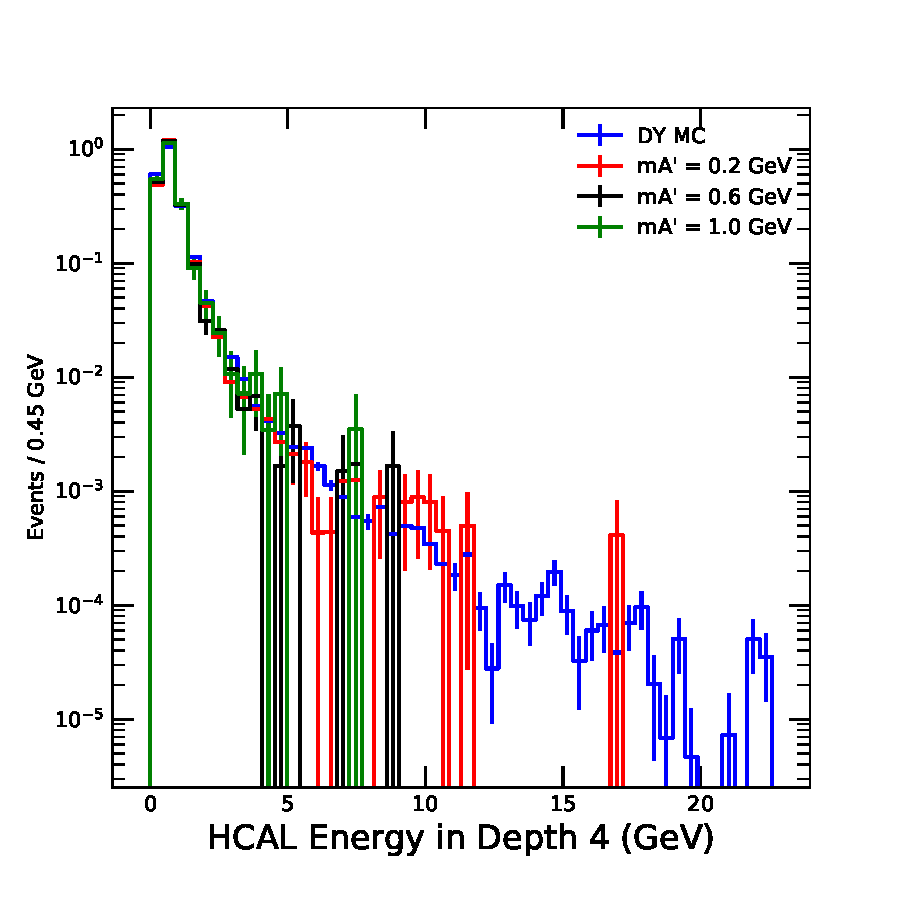
\includegraphics[width=0.45\textwidth]{figures/bdtInputFeatsHEDepth_4.pdf}
	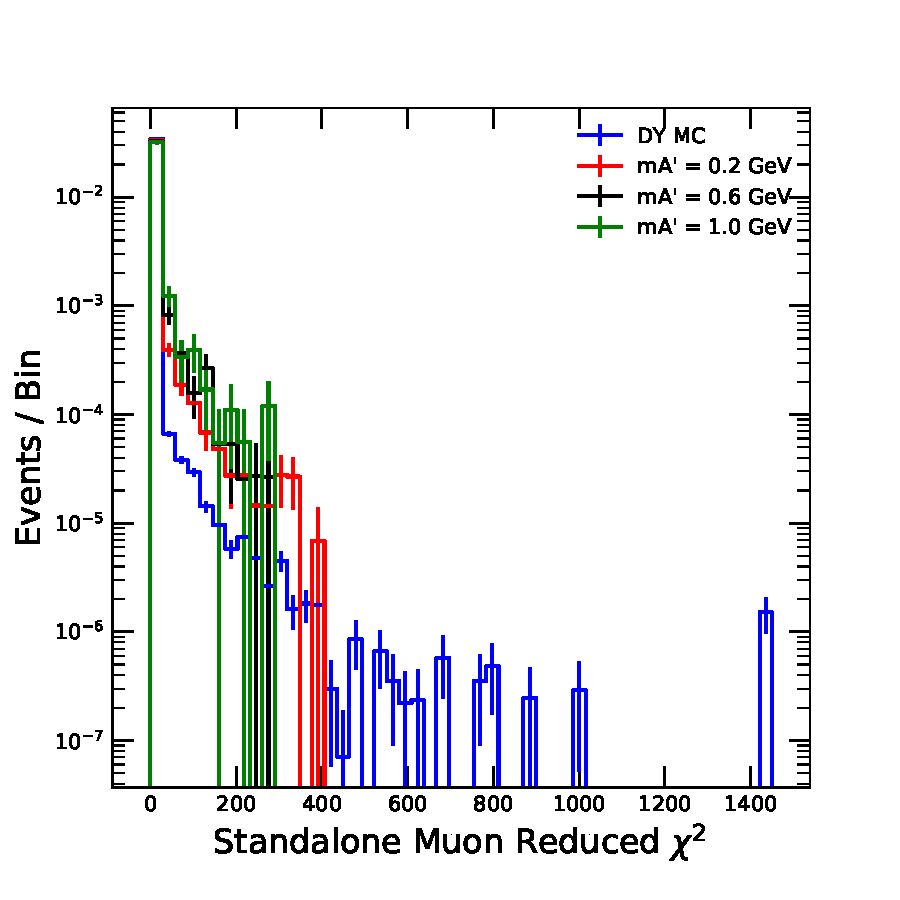
\includegraphics[width=0.45\textwidth]{figures/bdtInputFeatsstaChi.pdf}
	\hspace{0.01\textwidth}
	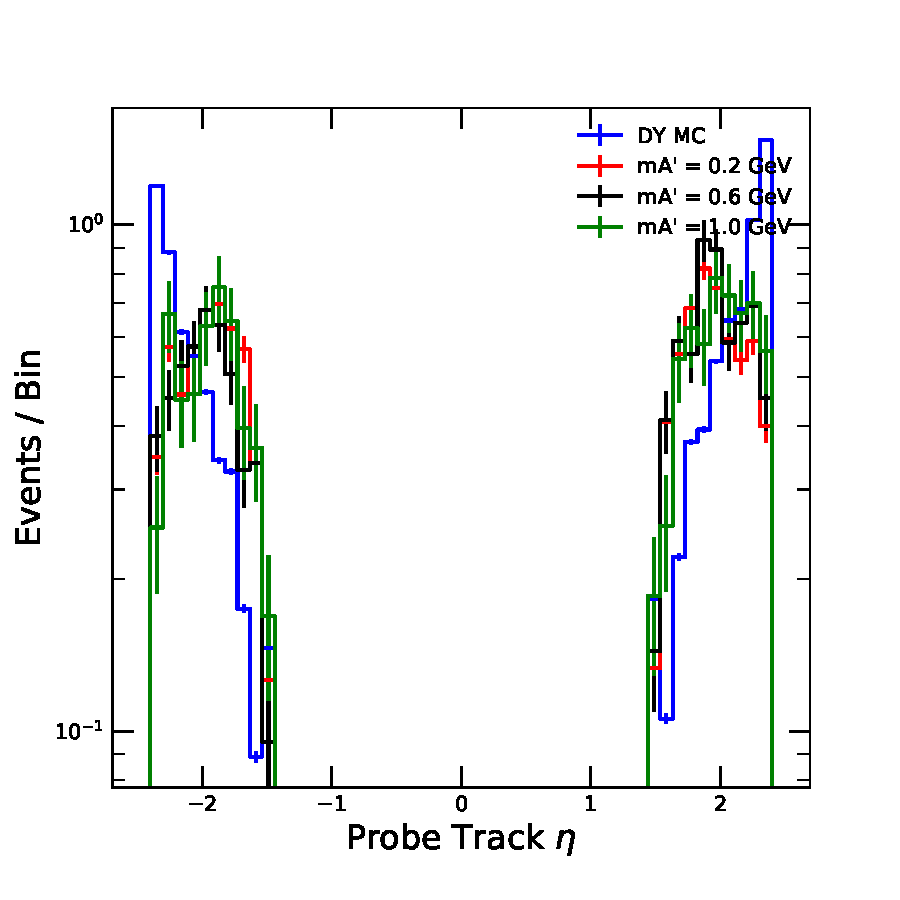
\includegraphics[width=0.45\textwidth]{figures/bdtInputFeatseta.pdf}
	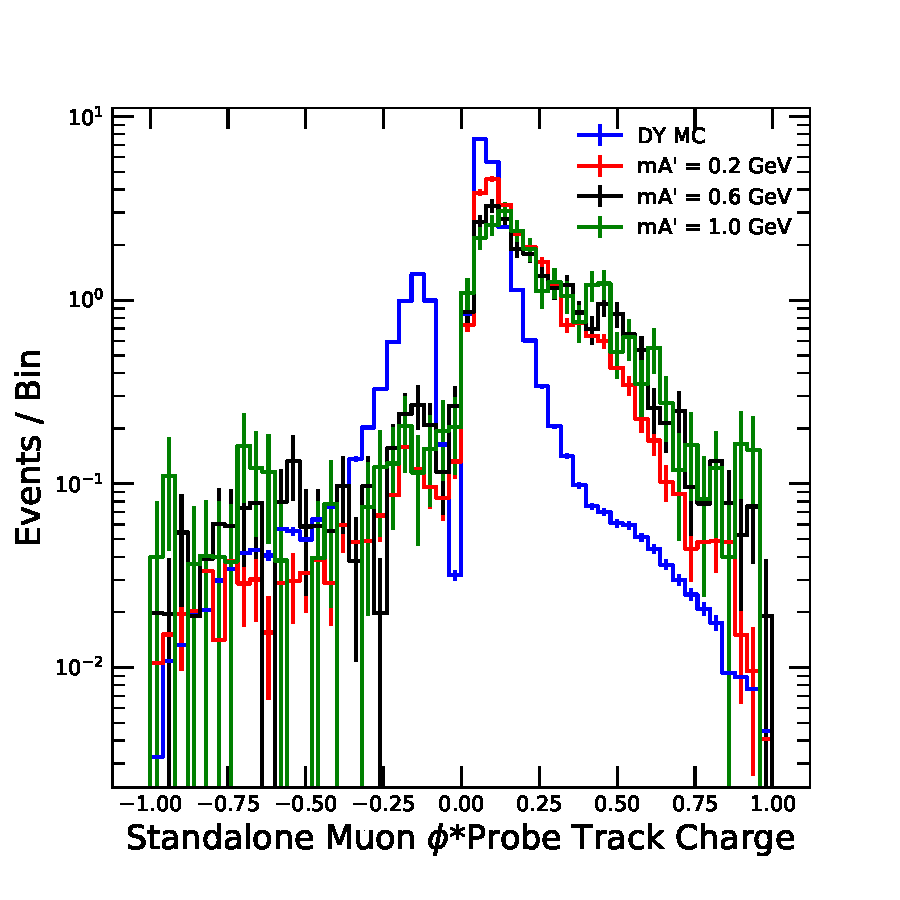
\includegraphics[width=0.45\textwidth]{figures/bdtInputFeatsstaPhi.pdf}
	\caption[Input BDT Classification Features]{The distributions of the highest-relevance input feature to the BDT for signal and DY MC events. While some variables, such as the CSC hit $\Delta$R and standalone muon $\Delta\phi$, have clear separation between signal and background, others have very similar behavior and are used to reject DY events with otherwise signal-like features based on correlations with their other inputs.}
	\label{fig:bdtFeatures}
\end{figure}

\section{Optimization}
A significant difficulty in training the partial region BDT is the imbalance between signal and background events. 
Because \dbrem is expected to be a rare process and large numbers of DY events pass the base event selection, many more background events are present than signal events and the background rejection rate must be prioritized over signal selection efficiency.

To represent this, signal events are given reduced weights to replicate their lower relative rate and increase the importance of background rejection.
Prior to optimization of the other parameters, a scan of this signal weight is made and the value which produces the strongest signal strength is selected.
To reduce the necessary validation and simplify the network, each signal mass is combined into one training input and weighted to give equal importance to each mass.

The internal parameters of the BDT are chosen using a randomized grid search, where each parameter is sampled from a flat distribution of possible values for a large number of trials.
To reduce the impact of overtraining in this parameter optimization, the training data is randomly split into five equally-sized independent subsets called \emph{folds}.
Five separate testing and training combinations sets are then defined, each with one fold used as a testing dataset and the other four used as a training dataset.

Five separate BDTs are then trained using these combinations.
During the training, only the training datasets are provided to the BDTs to prevent anomalous results from the network rejecting individual events based on non-generic event features.
The performance of the resulting BDTs is determined by their ability to correctly score their respective testing datasets, and the average weighted mean squared error of the five BDTs is used as the figure of merit in the randomized parameter search.
By selecting the parameters with the smallest average mean squared error the optimization can be performed while using the entire dataset to test the performance, as every event has a BDT which did not use it as training data, reducing the potential bias caused by the testing selection.

The parameters which are optimized during the grid search are the number of trees, the maximum tree depth, the fraction of each training sample used in each training stage, the weighting factor of each new tree, the loss reduction required to create new leaves, the fraction of input features used in each tree, the minimum weight in each node, and the strength of the regularization terms used in the objective function.

The output BDT score for DY MC and two representative A' masses is shown in \Cref{fig:BDToutput}. 
To reduce the sensitivity of the result to potential differences between the expected and observed BDT shape in DY events, a single signal bin is defined by selecting events with BDT scores $>$0.98 instead of using the BDT output shape in the final likelihood fits.
Lower A' masses typically have smaller deflections and energy loss, and therefore more background-like BDT scores than larger A' masses, but have increased sensitivity due to their larger \dbrem production cross sections.

\begin{figure}[htbp]
	\centering
	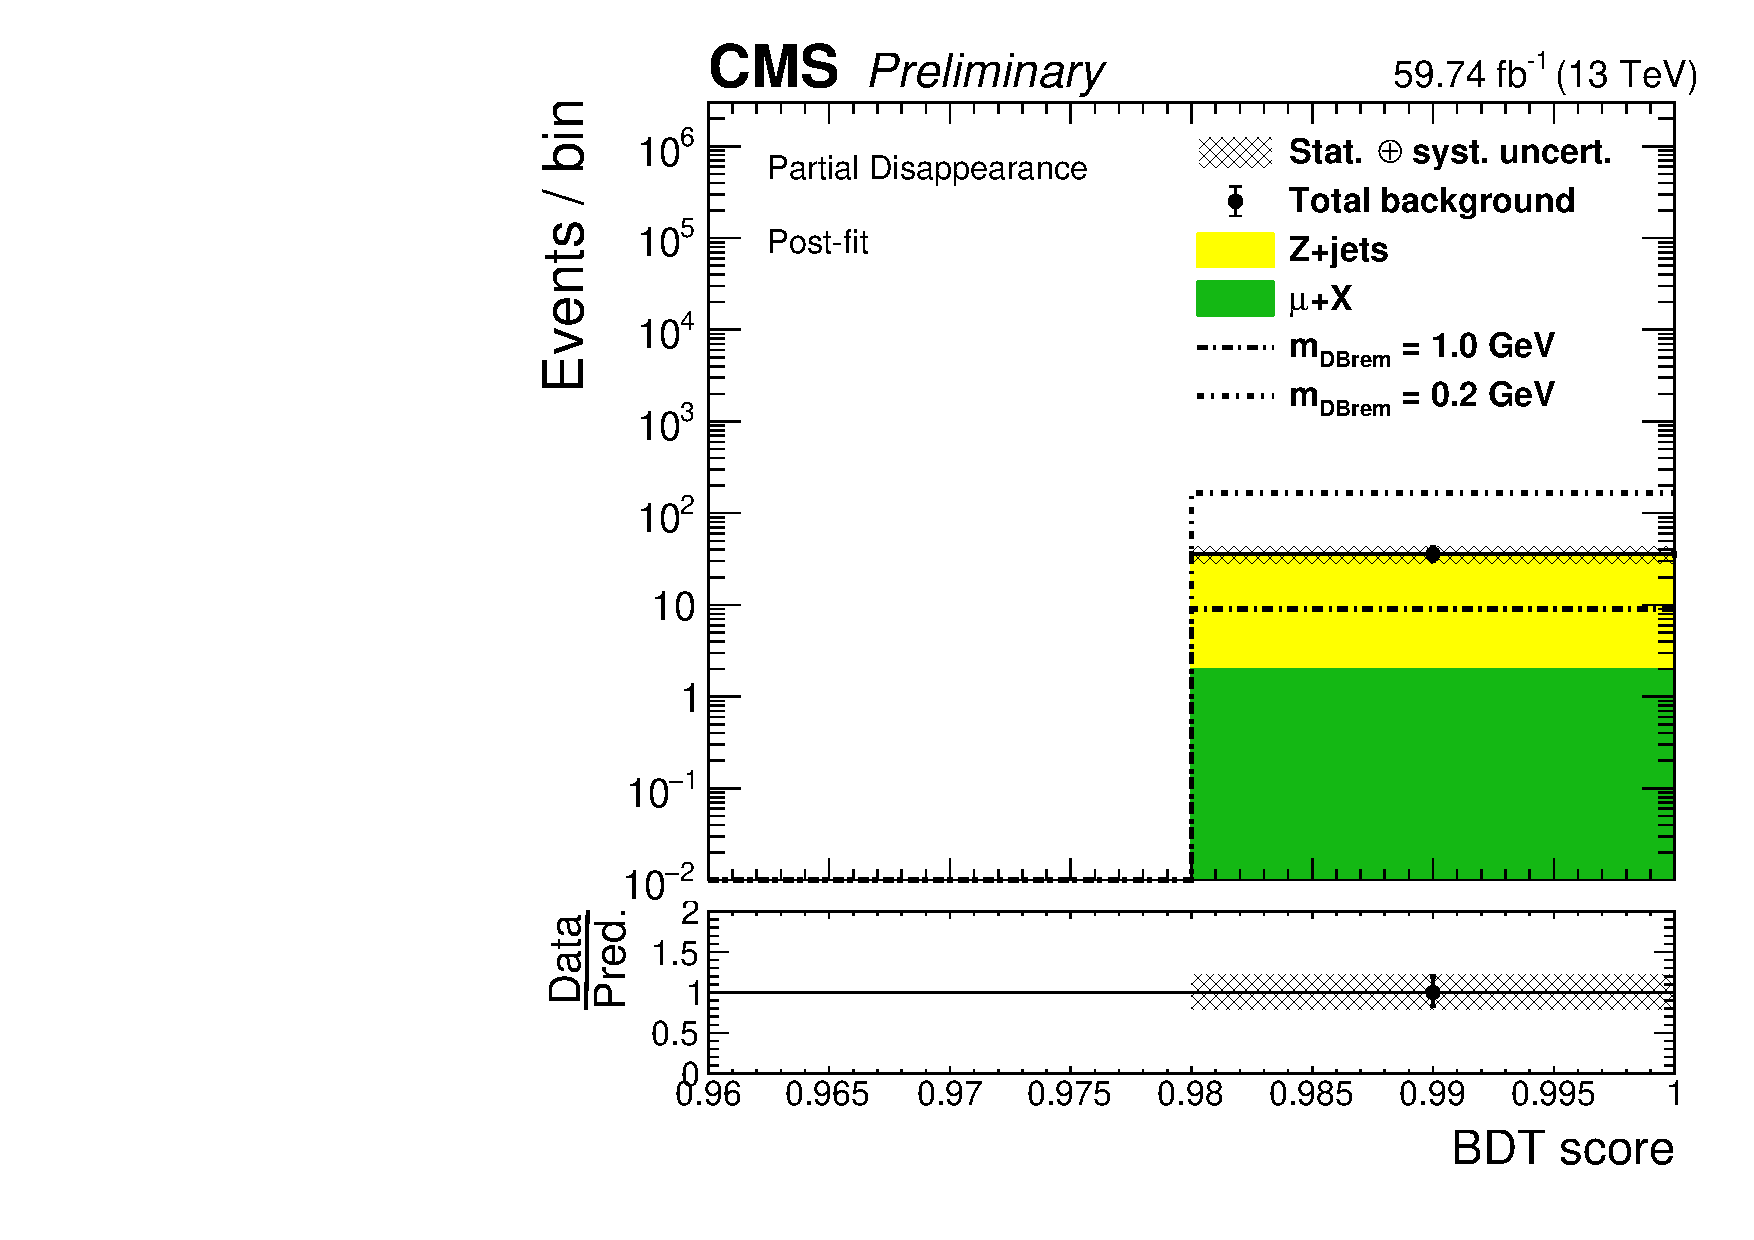
\includegraphics[width=0.9\textwidth]{figures/BDTscore_DYandSignal.pdf}
	\caption[Partial Disappearance BDT Output for DY and Signal]{The BDT score distribution of partial disappearance candidate events for DY MC (filled histogram) and signal (dashed line) samples. The hatched uncertainty bands on the simulated backgrounds indicate combined statistical and systematic components. Events in the highest bin, BDT score $>$0.98, form the signal region.}
        \label{fig:BDToutput}
\end{figure}

\section{Validation}
\label{sec:BDTvalid}
Two control regions are used to validate the performance of the BDT on background events, one consisting of probe tracks with large HCAL isolations ($>$\SI{30}{\giga\eV}), and one consisting of events with BDT scores less than 0.7. 
The HCAL energy requirement tends to select for muons which have significant SM scatters within the detector, and thus have more signal-like features in the muon chambers and more background-like features in the HCAL.

Events with poor HCAL isolation also select for $\mu+X$ backgrounds at a much larger rate than in the signal region.
In order to estimate their impact, data events with same-sign tag and probe pairs along with the same HCAL isolation threshold are used.
Though these events do not contain $\mu$+X backgrounds which may be produced by charge correlated processes, they can be used to provide an estimate for the distribution and relative scale of the overall $\mu+X$ background.

The distributions of the standalone muon $\Delta$E/E, $\chi^{2}$, and $\Delta\phi$ are shown in \Cref{fig:BDTstavalid}. 
Differences between data and MC are observed for some regions of all three variables, particularly at low muon energy, high standalone muon reduced $\chi^{2}$, and $\Delta\phi$ with magnitude near 0.2. 
These differences are uncorrelated with muon charge, and are likely produced by inefficiency in CSC reconstruction which results in lower-quality standalone muon fits.

\begin{figure}[htbp]
	\centering
	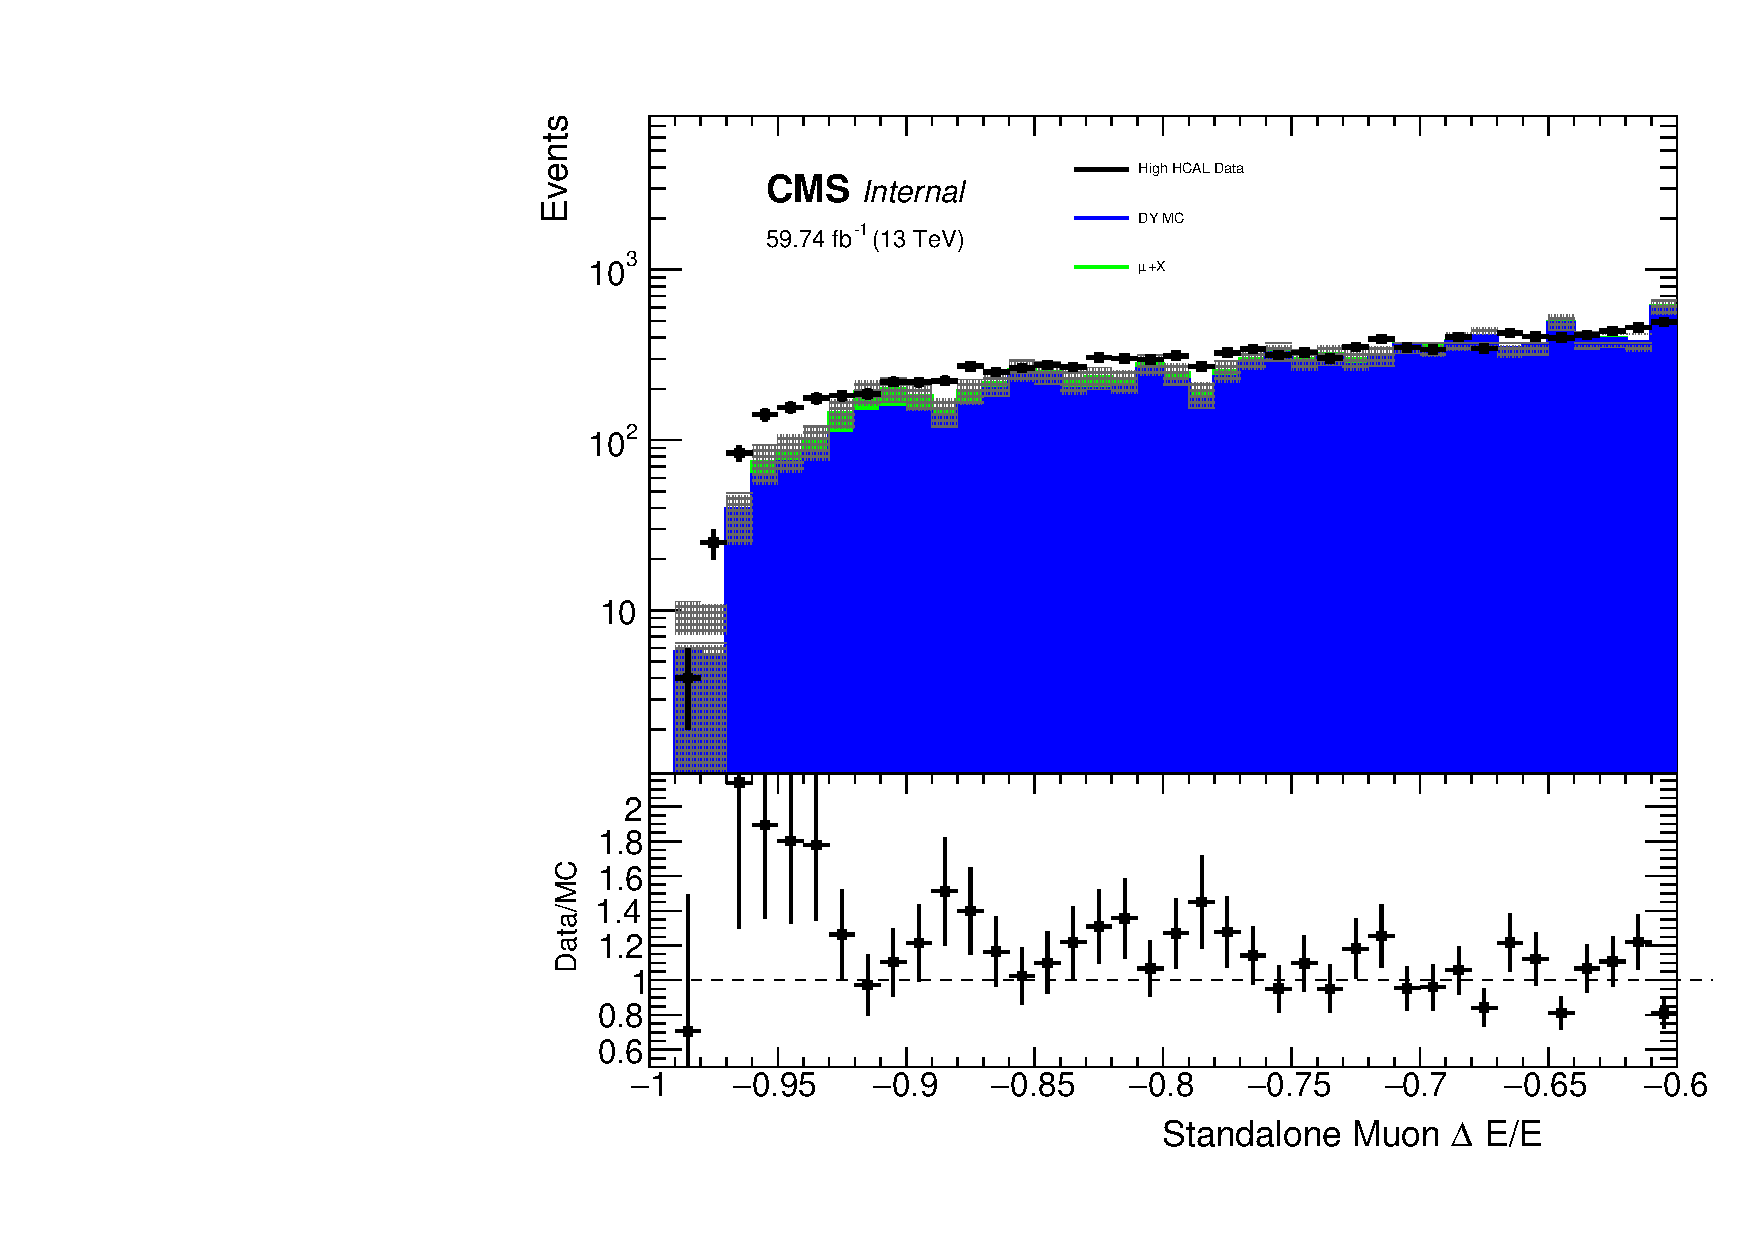
\includegraphics[width=0.45\textwidth]{figures/standaloneMuonValidation.pdf}
	\hspace{0.01\textwidth}
	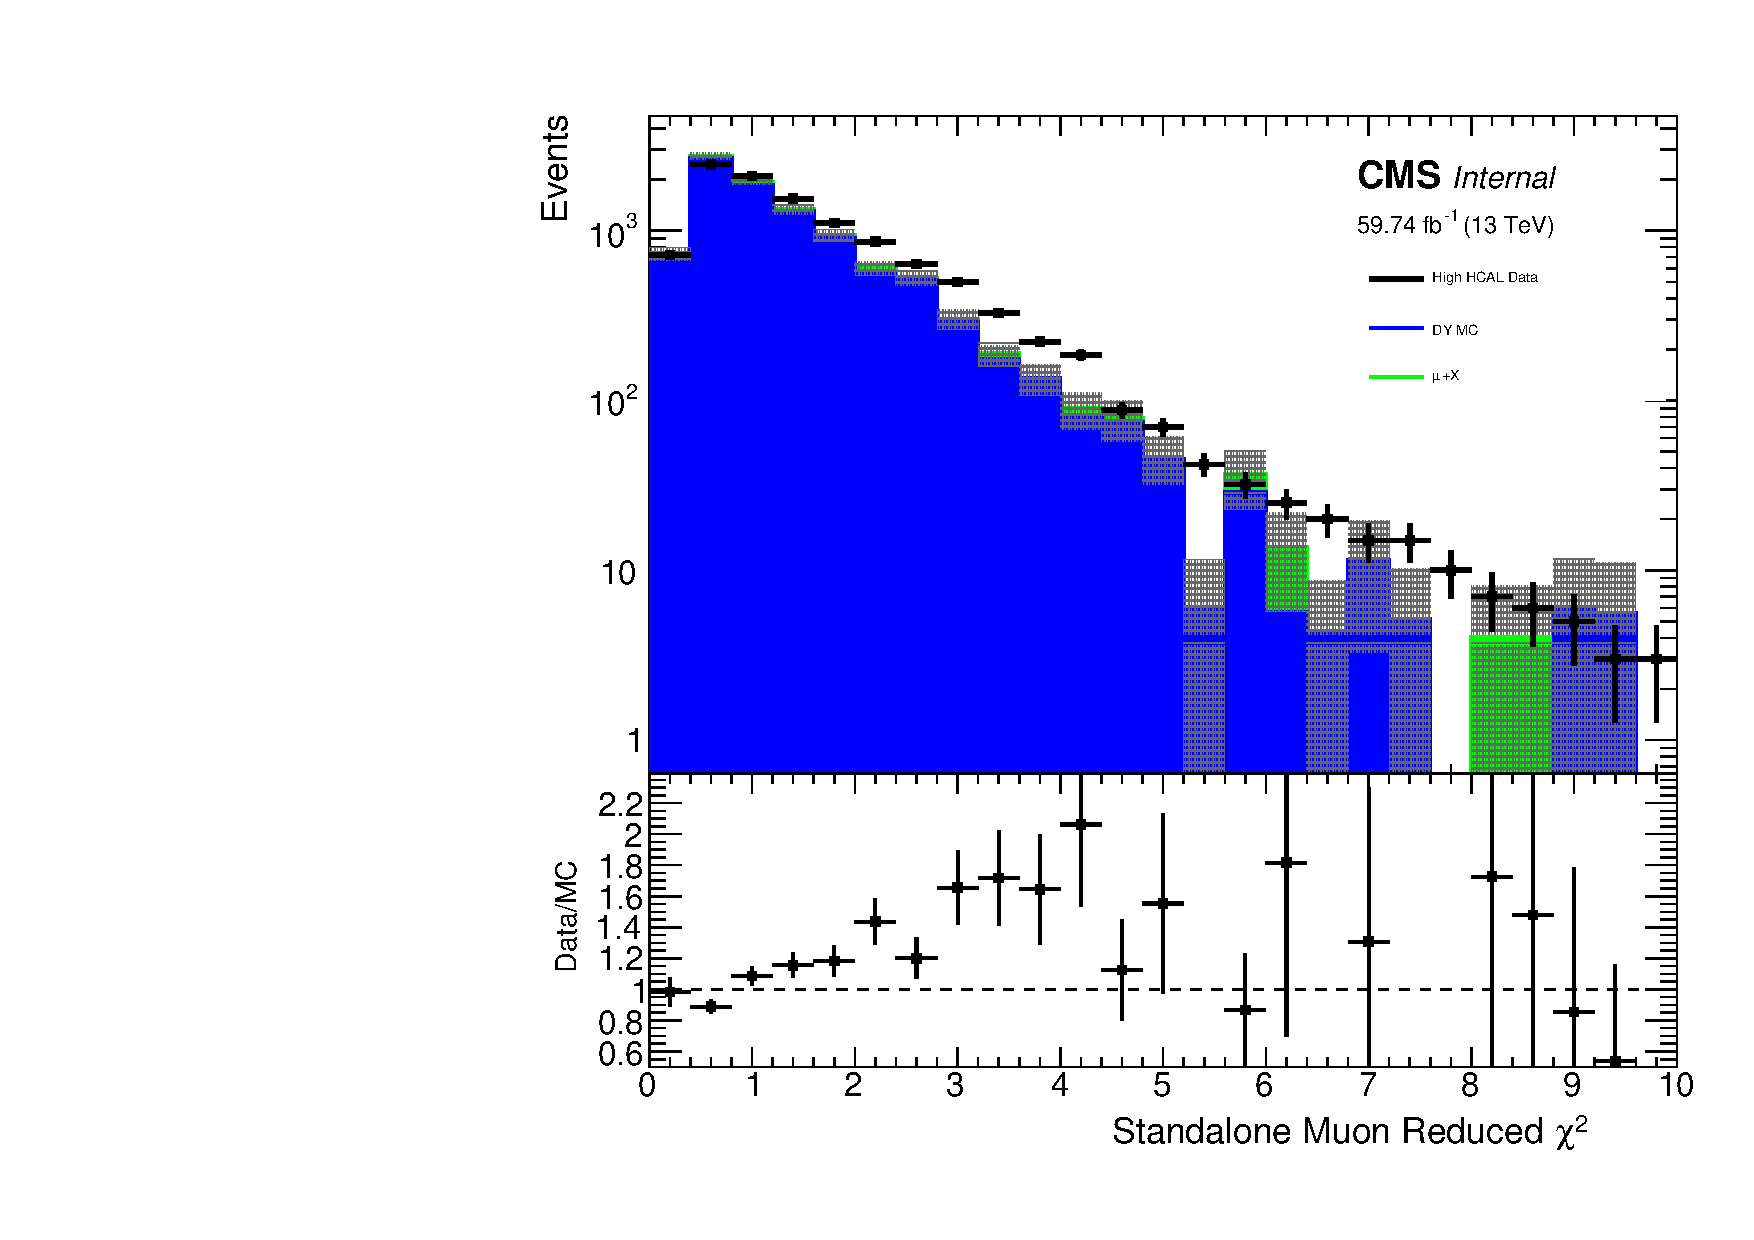
\includegraphics[width=0.45\textwidth]{figures/standaloneMuonChiValidation.pdf}
	\vspace{0.01\textwidth}
	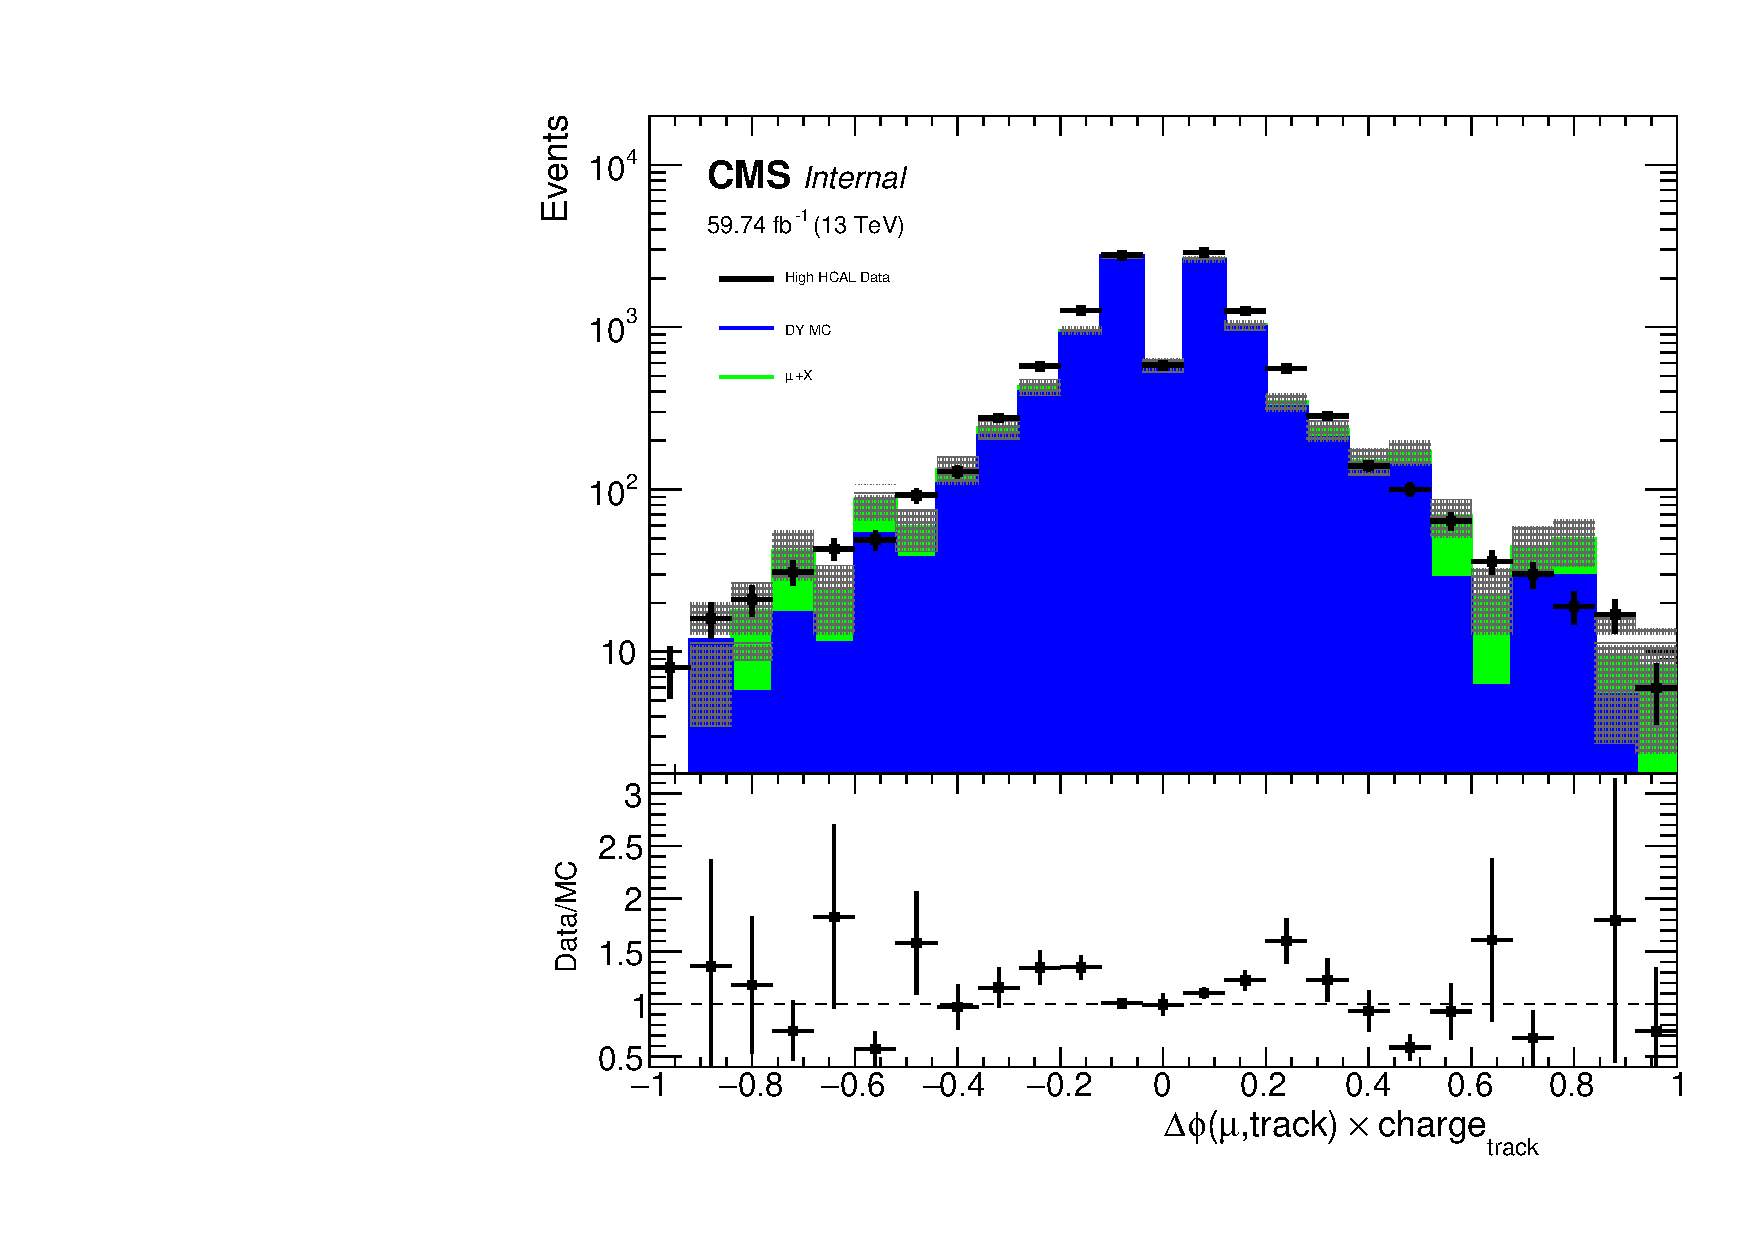
\includegraphics[width=0.45\textwidth]{figures/standaloneMuonPhiValidation.pdf}
        \caption[Standalone Muon Validation]{Standalone muon variables used as inputs to the partial region BDT measured in the high HCAL energy control region. Discrepancies are present in events with very low standalone muon $\Delta$E/E, large reduced $\chi^{2}$, and $\Delta\phi$ of $\sim|$0.2$|$.}
        \label{fig:BDTstavalid}
\end{figure}

The distributions of the distance to the nearest CSC hit in each muon station are presented in \Cref{fig:BDTcscvalid}. 
Some differences between MC and data are observed in the CSC $\Delta$R distributions as well. 
As with the tag-muon aligned segments, the first CSC station has significant excesses of events with large $\Delta$R to the nearest hit and no nearby hits, while the other three depths have better overall agreement but overestimate the rates of events with intermediate $\Delta$R to the nearest CSC segment in the range of 0.1 to 2.

\begin{figure}[htbp]
	\label{fig:BDTcscvalid}
	\centering
	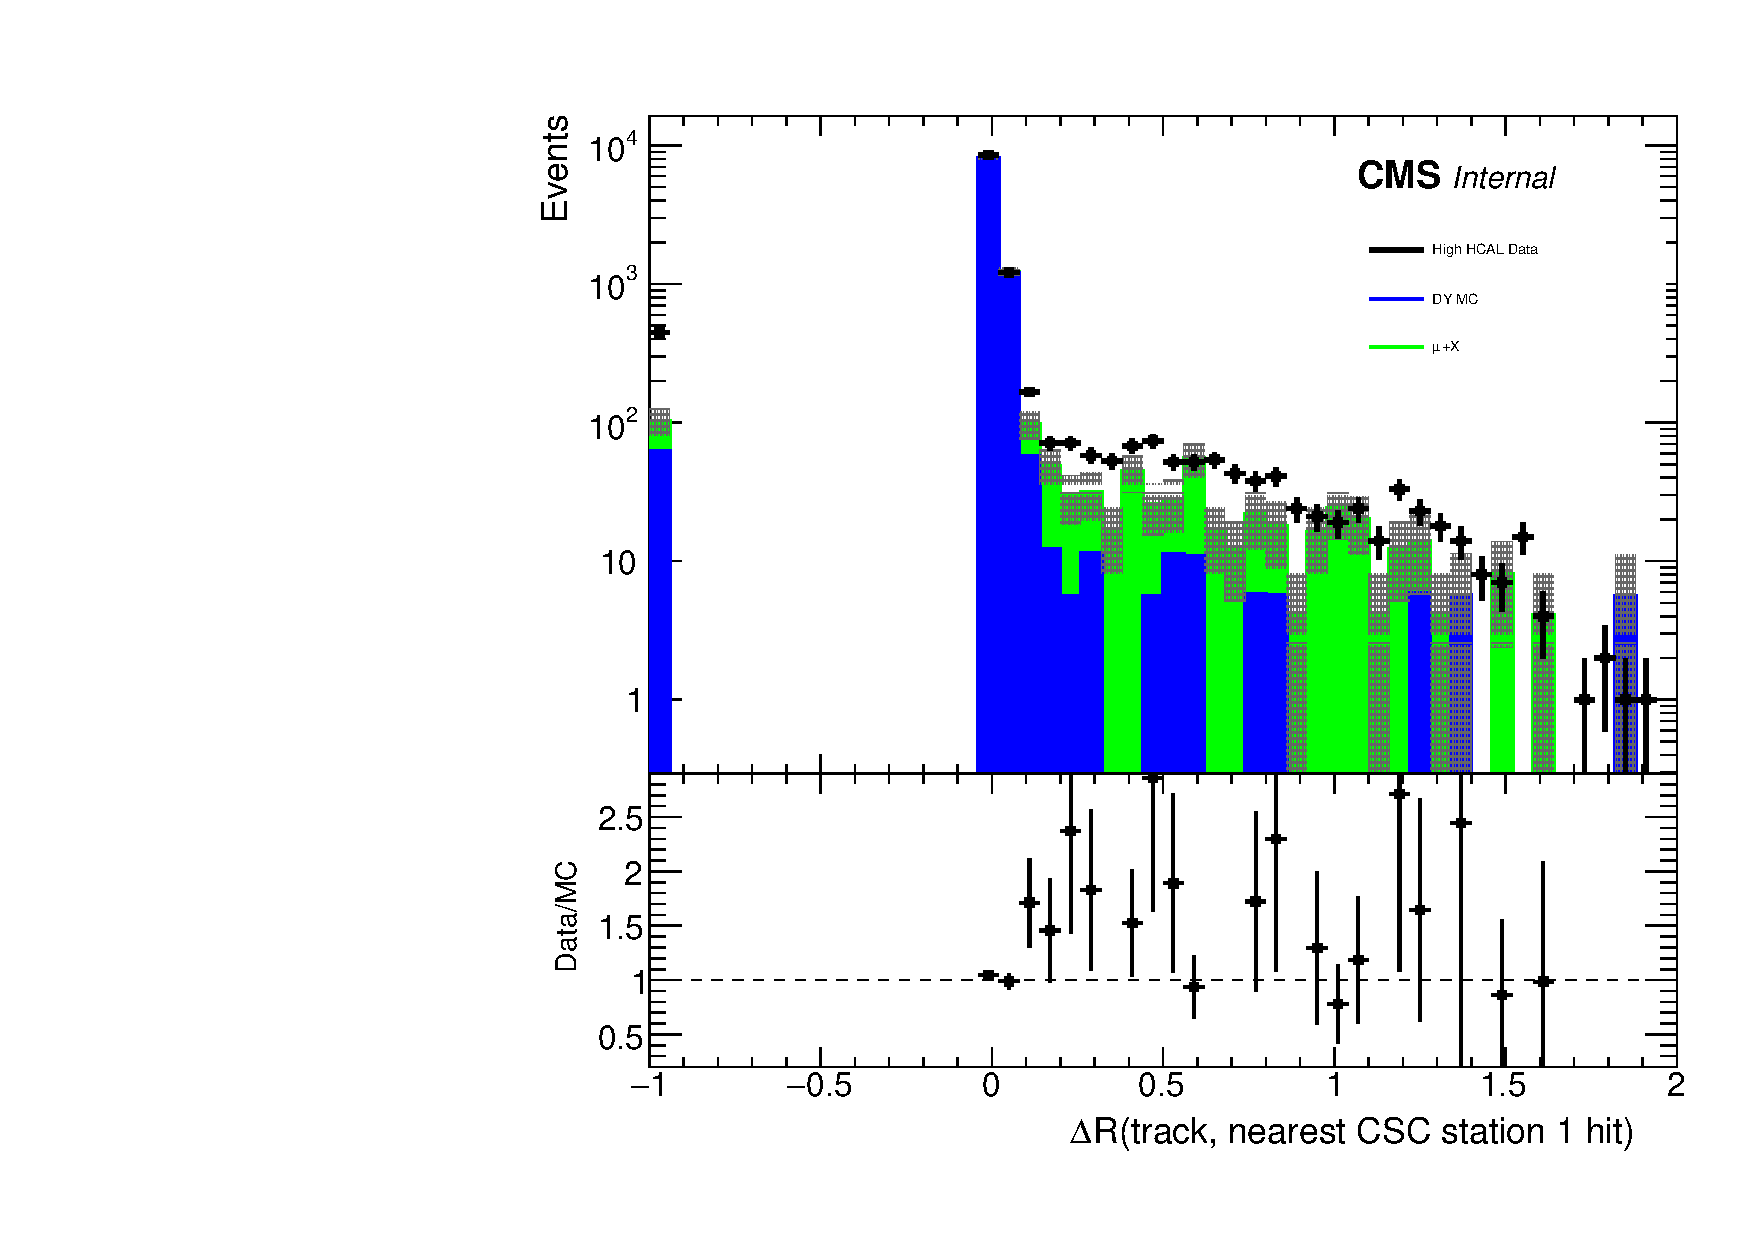
\includegraphics[width=0.45\textwidth]{figures/highHcal_cscDr_station0.pdf}
	\hspace{0.01\textwidth}
	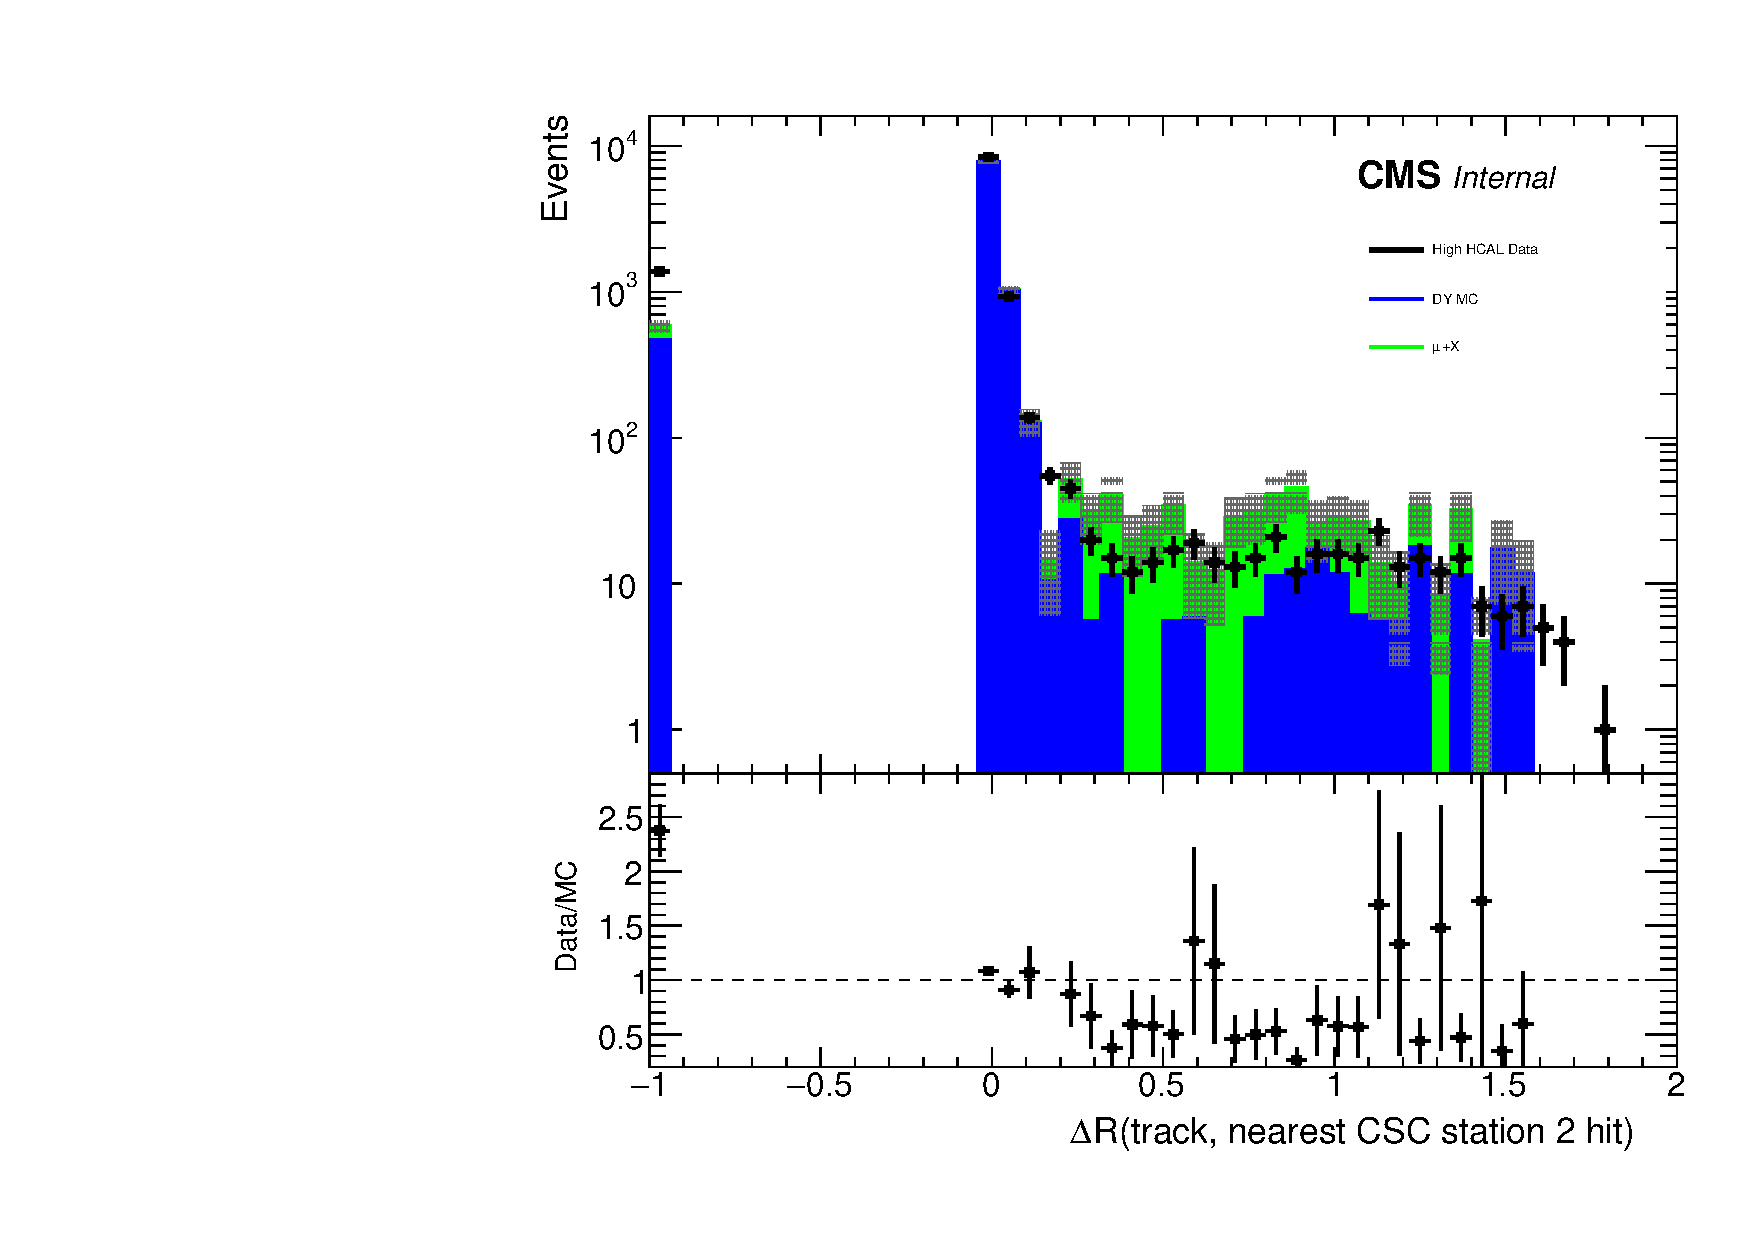
\includegraphics[width=0.45\textwidth]{figures/highHcal_cscDr_station1.pdf}
	\vspace{0.01\textwidth}
	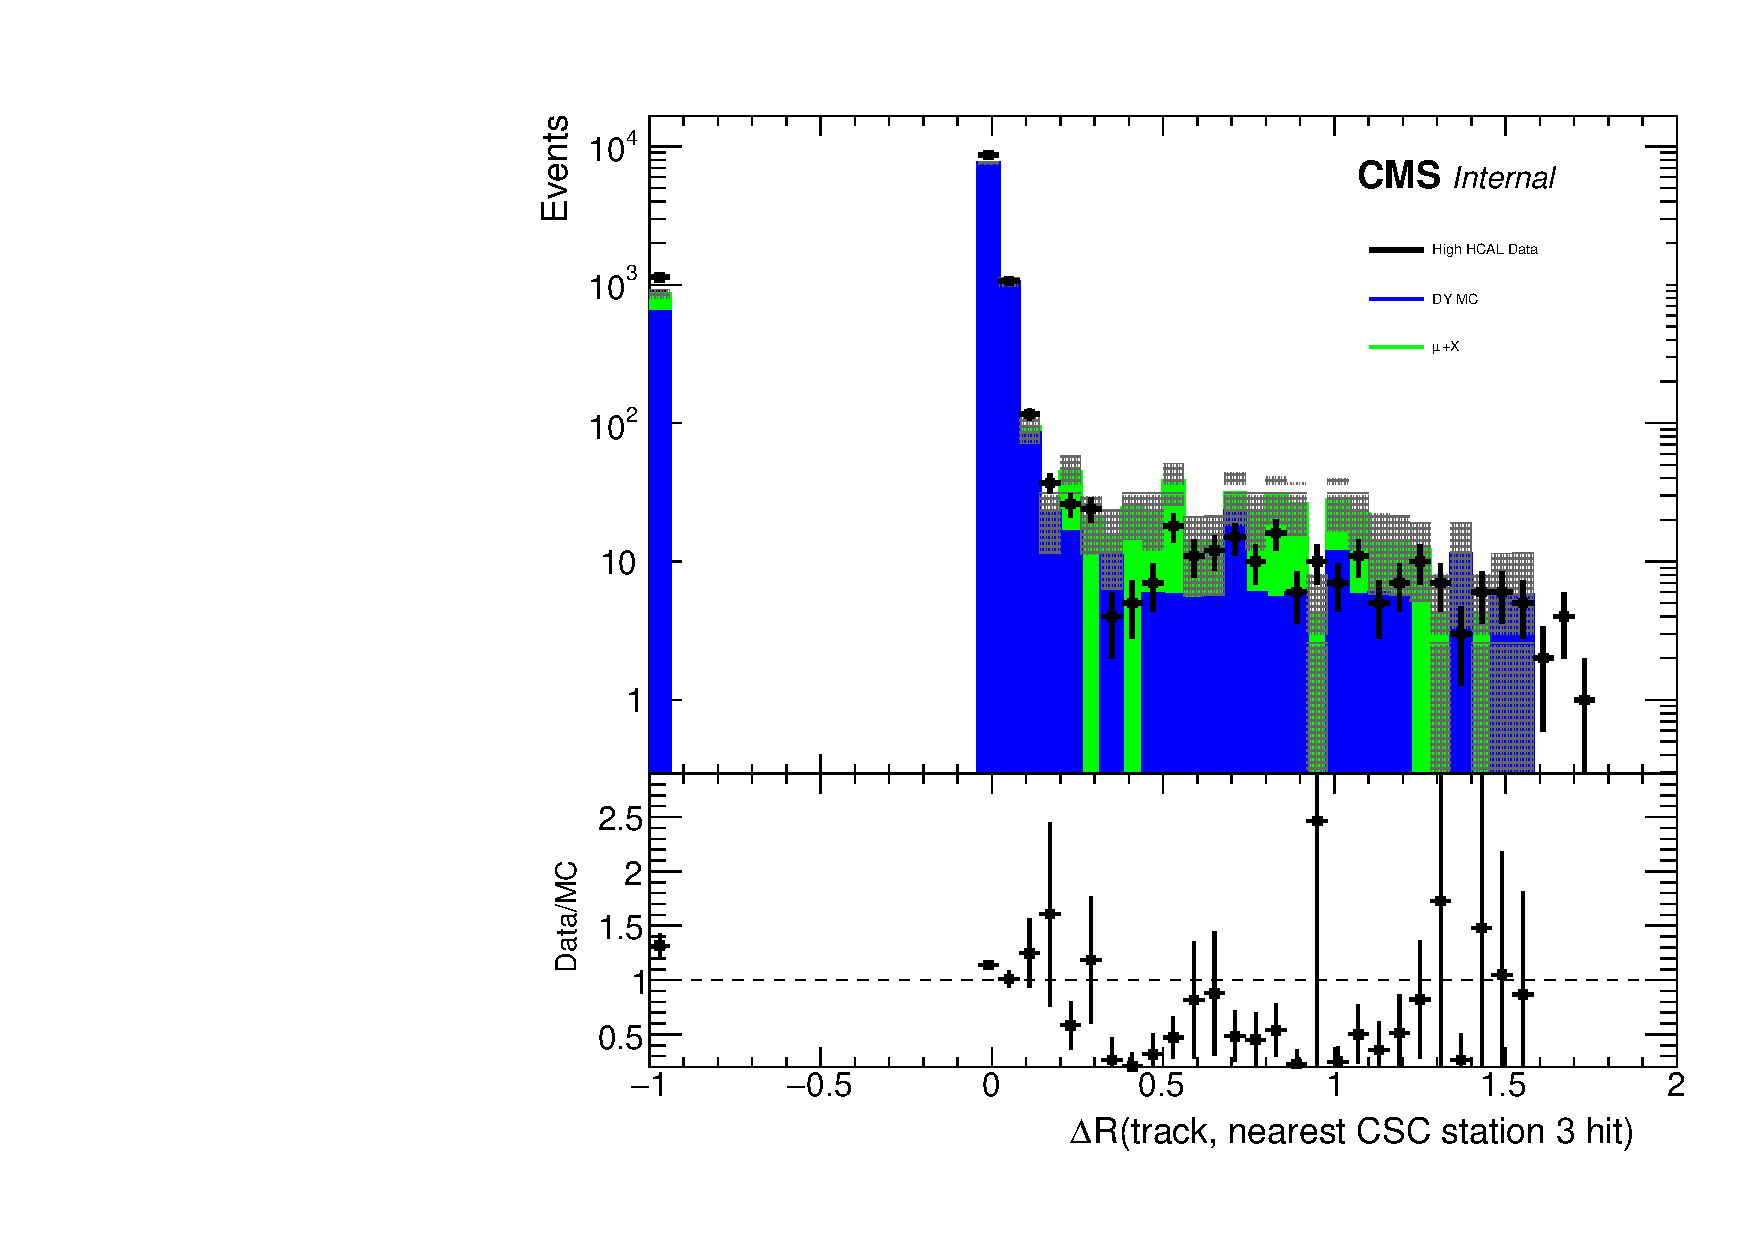
\includegraphics[width=0.45\textwidth]{figures/highHcal_cscDr_station2.pdf}
	\hspace{0.01\textwidth}
	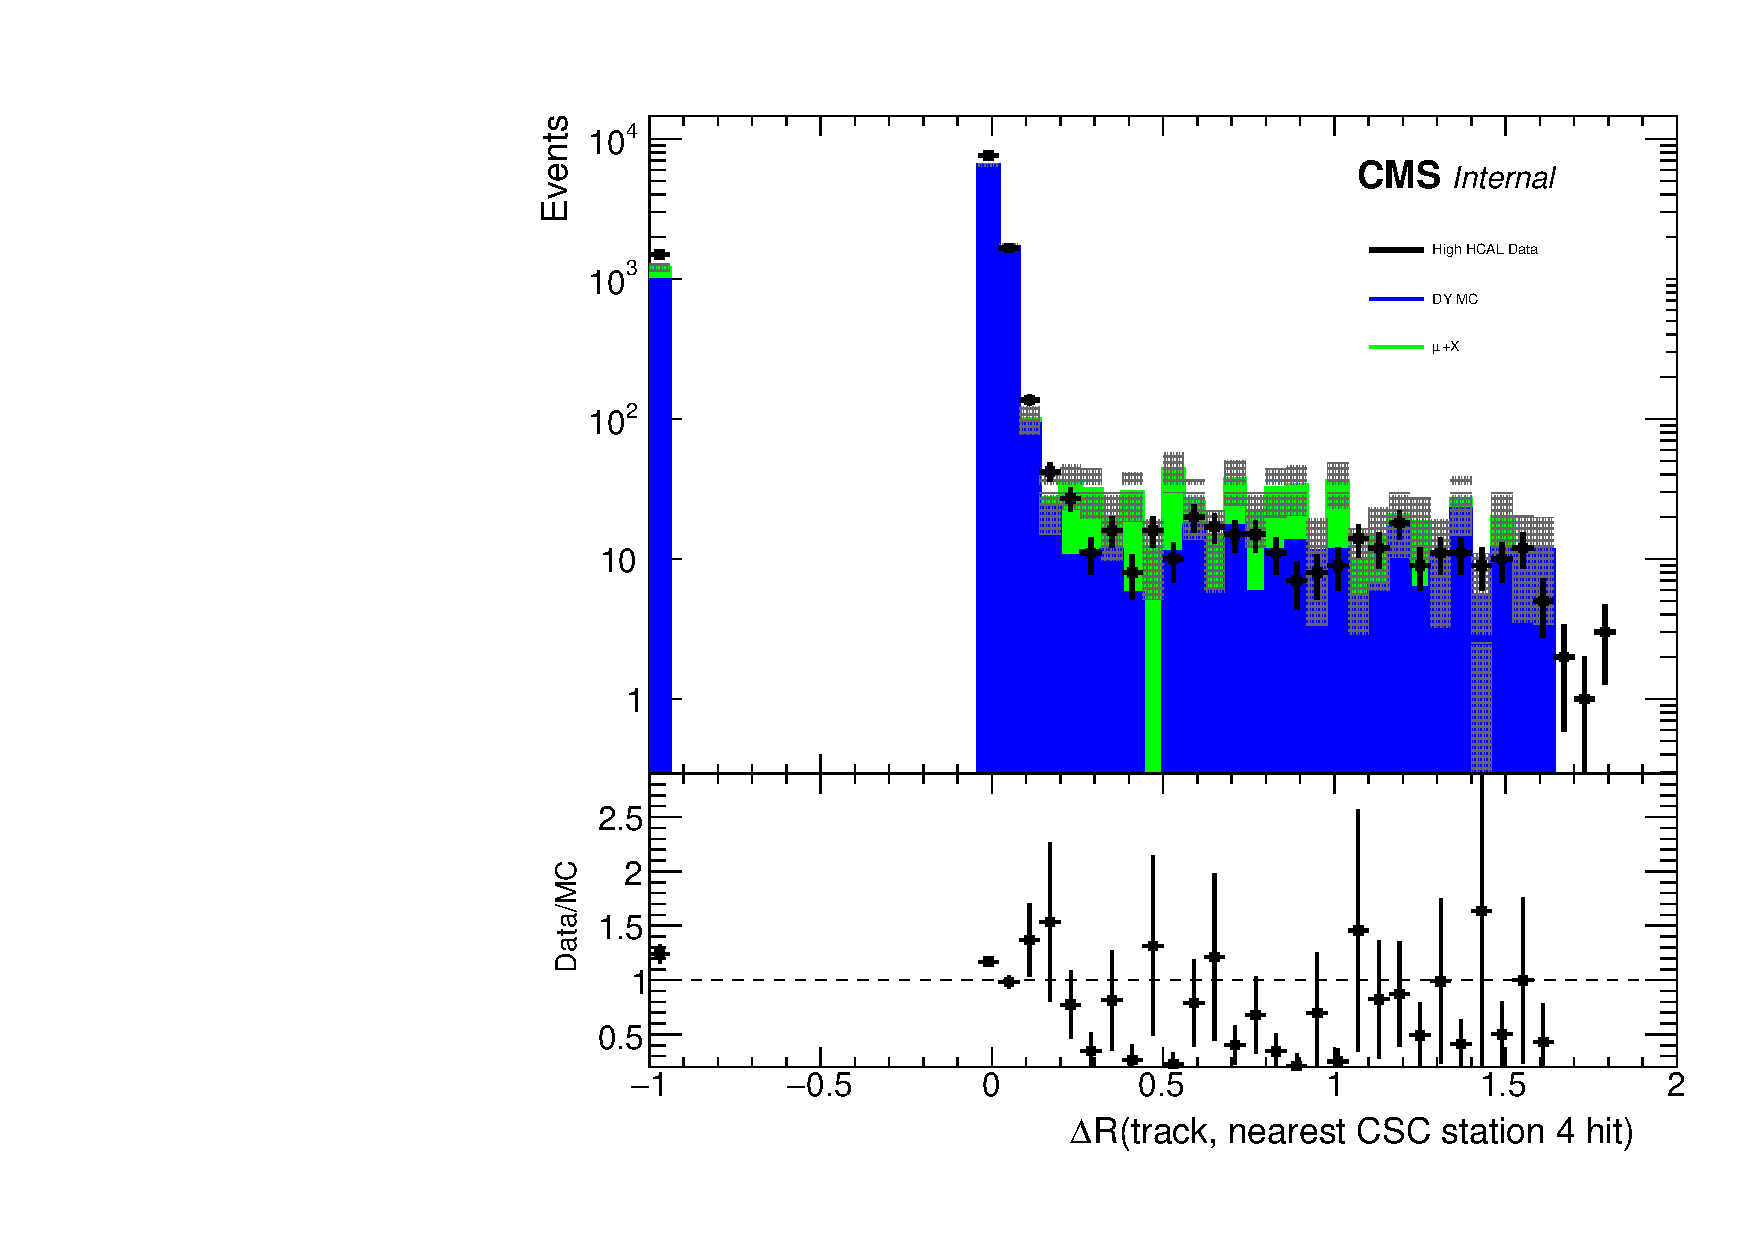
\includegraphics[width=0.45\textwidth]{figures/highHcal_cscDr_station3.pdf} 
        \caption[CSC Segment Validation]{The distance to the nearest CSC segment in each station measured along the probe track trajectory for partial disappearance events in the high HCAL energy control region. Events with no CSC hits in a station within $\Delta$R$<$2 are assigned a value of -1.}
\end{figure}

The BDT scores of events in this region for data and MC are shown in \Cref{fig:BDTscorevalid}.
As expected, the region is relatively shifted to higher BDT scores than DY events which are isolated in HCAL due to the more signal-like event features in this region produced by energy loss to standard model processes in the HCAL. 

\begin{figure}[htbp]
	\label{fig:BDTscorevalid}
	\centering
	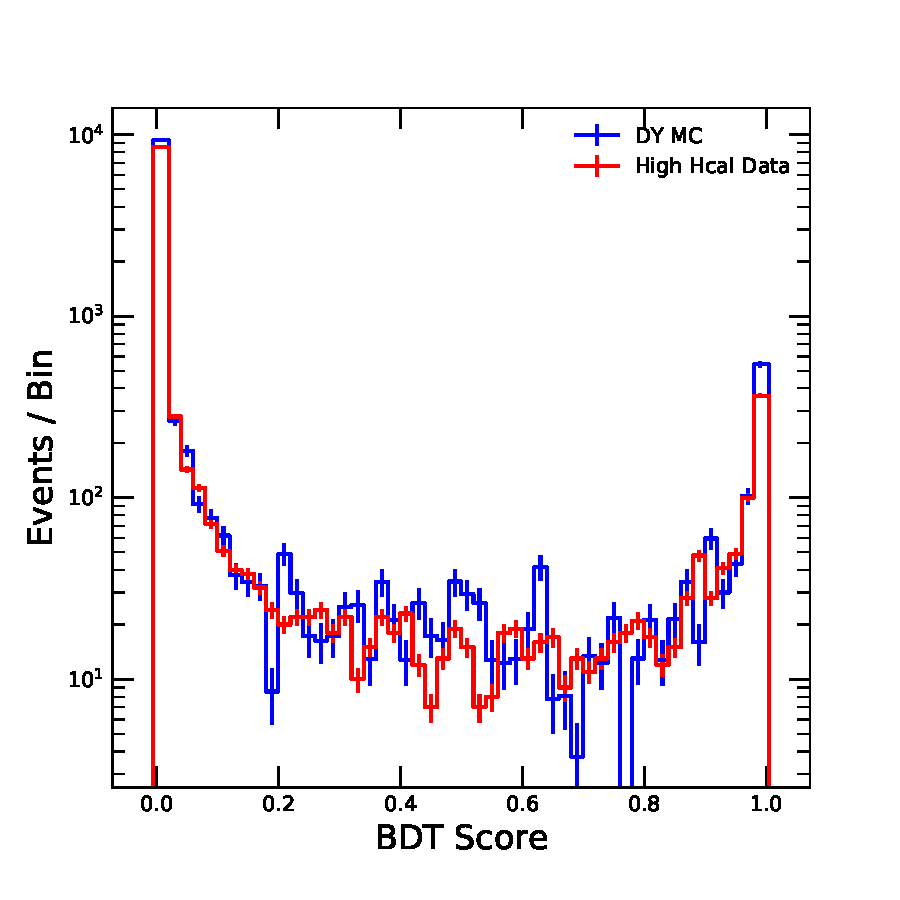
\includegraphics[width=0.6\textwidth]{figures/highHcalValid.pdf}
        \caption[BDT Validation in the High HCAL Energy Control Region]{The distribution of BDT scores for data and DY MC events in the high HCAL control region.}
\end{figure}

While good agreement is seen in high-HCAL energy events with intermediate scores, an excess of simulated events in the signal region (BDT score $>$0.98) is observed.
Because of the difference in event features between the signal region and the high-HCAL control region, this difference cannot be used to directly derive scale factors to correct MC, but instead is applied as a systematic uncertainty on the expected rate of DY background.
Though this region produces a deficit of background events, this uncertainty is allowed to either increase or decrease the expected rate, using the observed difference as an estimate of the magnitude of change that might be present.

In contrast to the high-HCAL energy region, events with low BDT scores (BDT score $<0.7$) contain background-like features in both the CSCs and HCAL and can be used to validate the simulation of the DY backgrounds as well as the performance of the BDT on these events.
In initial studies of this region, significant differences were observed in several features related to the standalone muons, with excess events containing large $\Delta$R to the nearest standalone muon, low standalone muon energy, and large trajectory change between the probe track and the nearest standalone muon \Cref{fig:lowScoreVariableMismatch}.

\begin{figure}[htbp]
	\label{fig:lowScoreVariableMismatch}
	\centering
	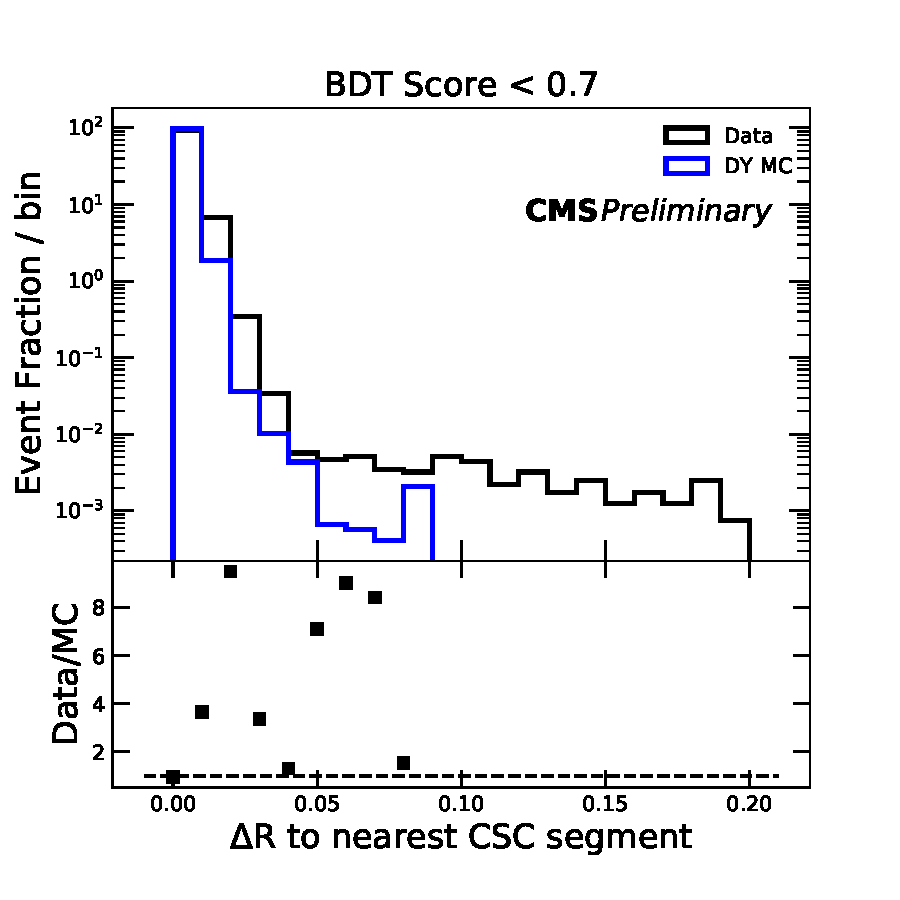
\includegraphics[width=0.45\textwidth]{figures/badPartialRegioncscDR.pdf}
	\hspace{0.01\textwidth}
	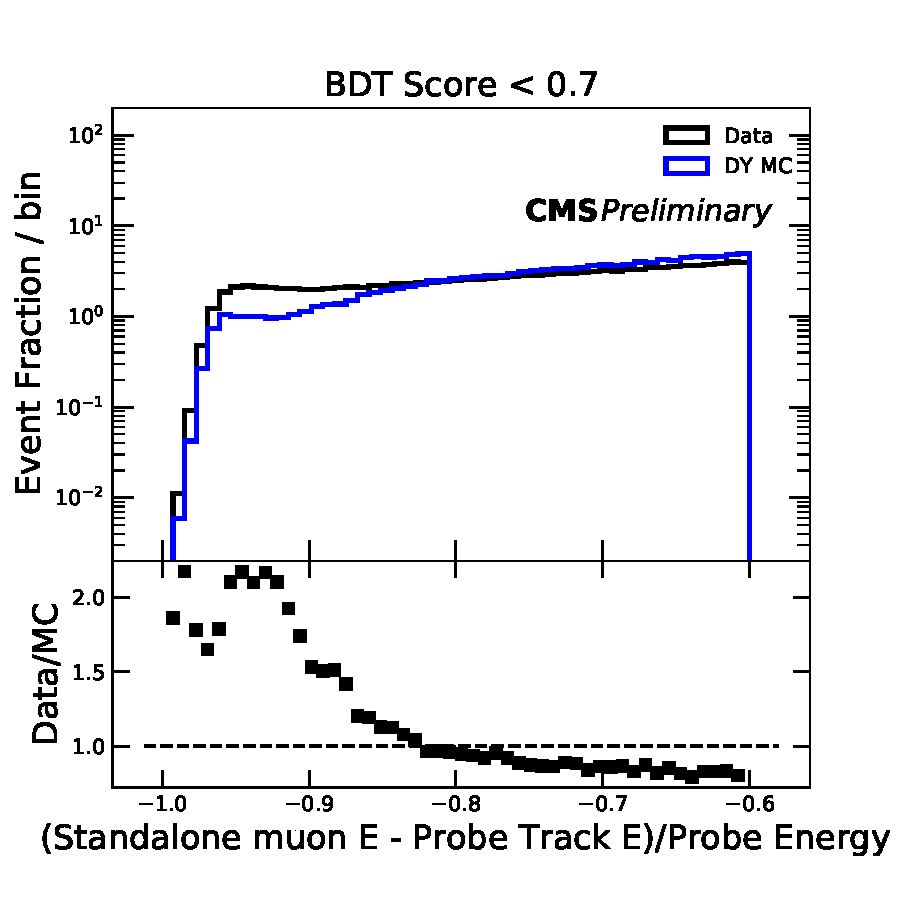
\includegraphics[width=0.45\textwidth]{figures/badPartialRegionstandaloneDEoverE.pdf}
	\vspace{0.01\textwidth}
	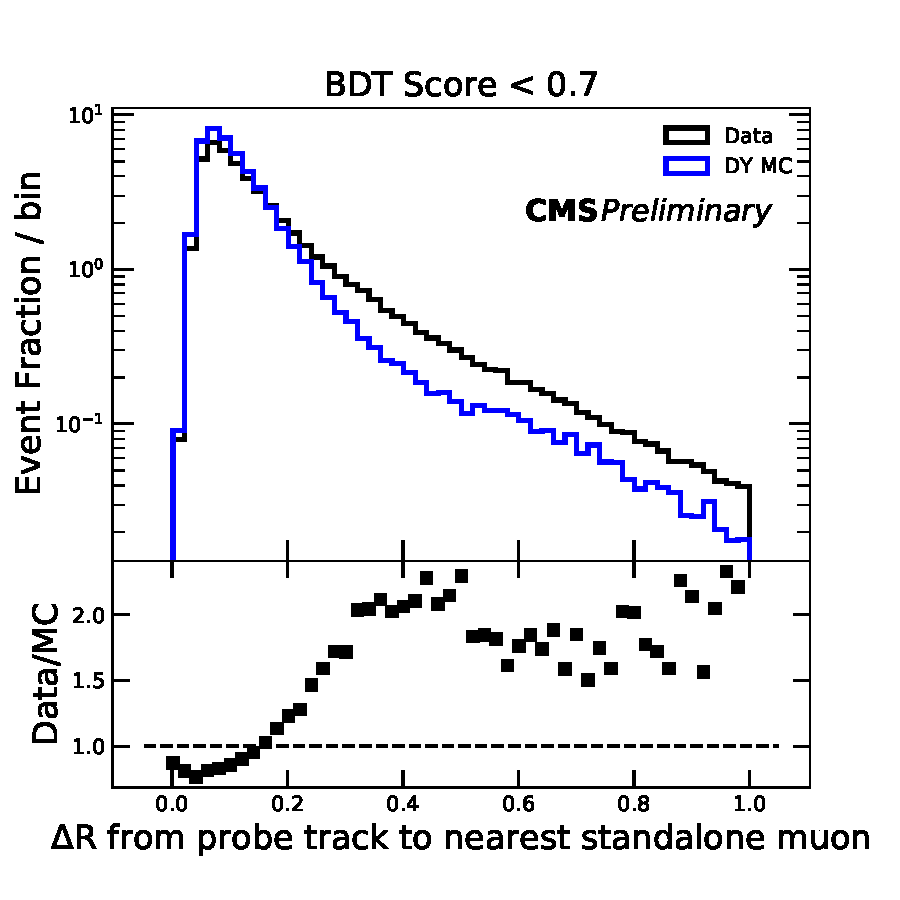
\includegraphics[width=0.45\textwidth]{figures/badPartialRegionstaDR.pdf}
	\hspace{0.01\textwidth}
	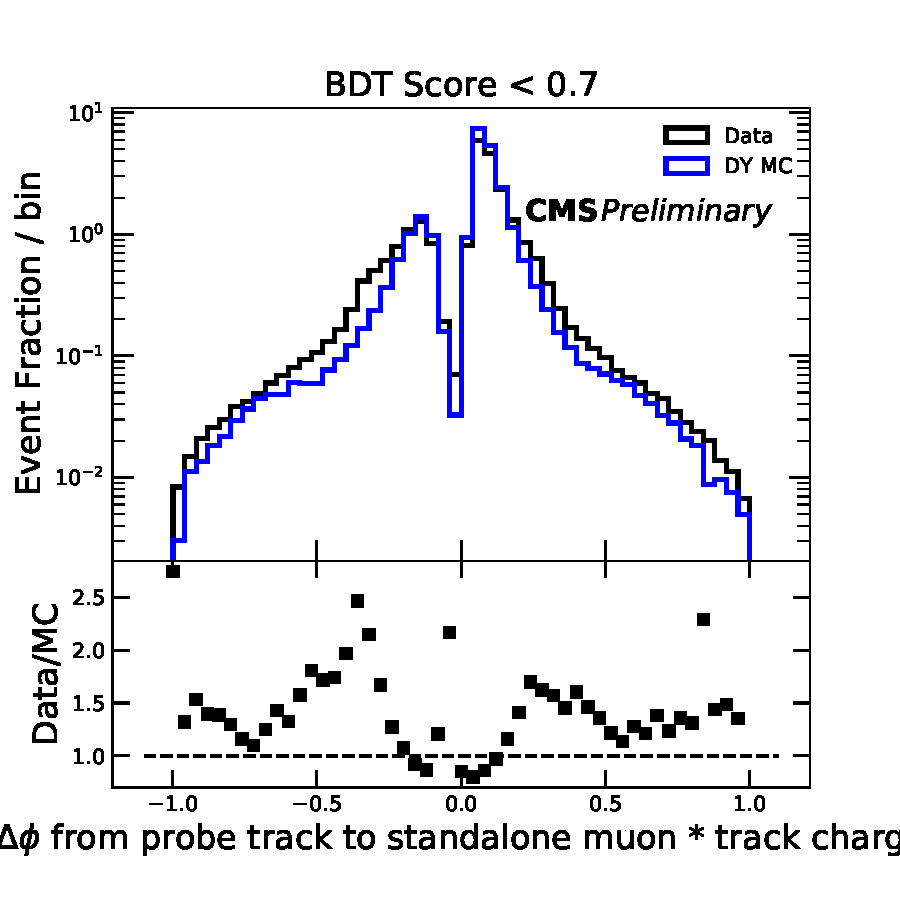
\includegraphics[width=0.45\textwidth]{figures/badPartialRegionstaPhi.pdf} 
        \caption[Low-Score Event Validation Before Correction]{Input features showing significant differences between data and DY simulation in the low BDT score control region prior to the rejection of low-quality standalone muons.}
\end{figure}

In addition, large differences in the overall normalization were observed between the data events and the expected rate of DY backgrounds, with nearly twice as many events selected as expected.
Through study of these anomalous events, it was found that they correspond to cases where large differences in CSC segment position were present between the first CSC station and the later three.
These position differences cause the reconstruction of the standalone muon to produce anomalously low energy and altered trajectories, resulting in several signal-like differences in the final objects. 

Large positional differences between the first and later CSC stations are not frequently seen in signal events, as energy loss within the HCAL results in significant deflection before reaching the CSC chambers but relatively small deflection from station to station. 
As a result, these anomalous standalone muons can be removed using quality requirements based on the $\Delta$R of the nearest CSC segments in stations two, three, and four to the position of the nearest CSC segment in the first CSC station.
After removing events with no CSC segments in the later stations within $\Delta\mathrm{R}<0.04$ of the nearest CSC segment in station one, significant improvement is seen in the individual standalone muon features (\Cref{fig:lowScoreInputCorrection}).
The overall normalization after this additional requirement differs by $8\%$, roughly in expectation with the combined cross section, luminosity, and selection efficiency uncertainties.

\begin{figure}[htbp]
	\label{fig:lowScoreInputCorrection}
	\centering
	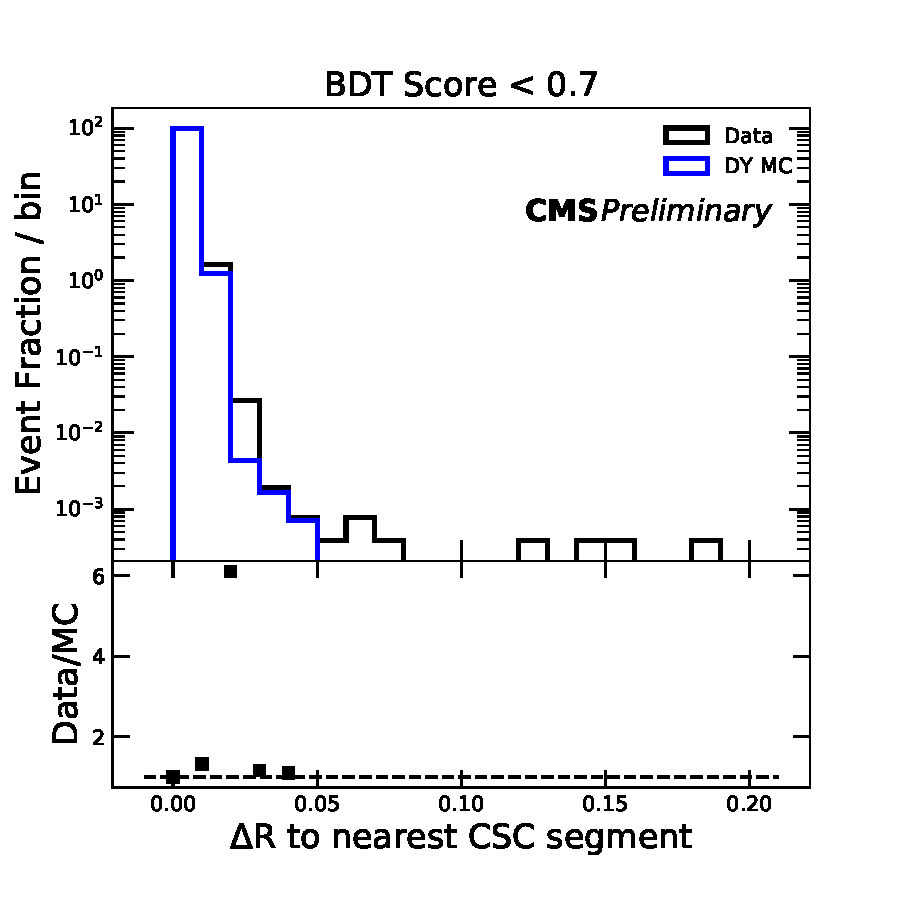
\includegraphics[width=0.45\textwidth]{figures/partialRegioncscDR.pdf}
	\hspace{0.01\textwidth}
	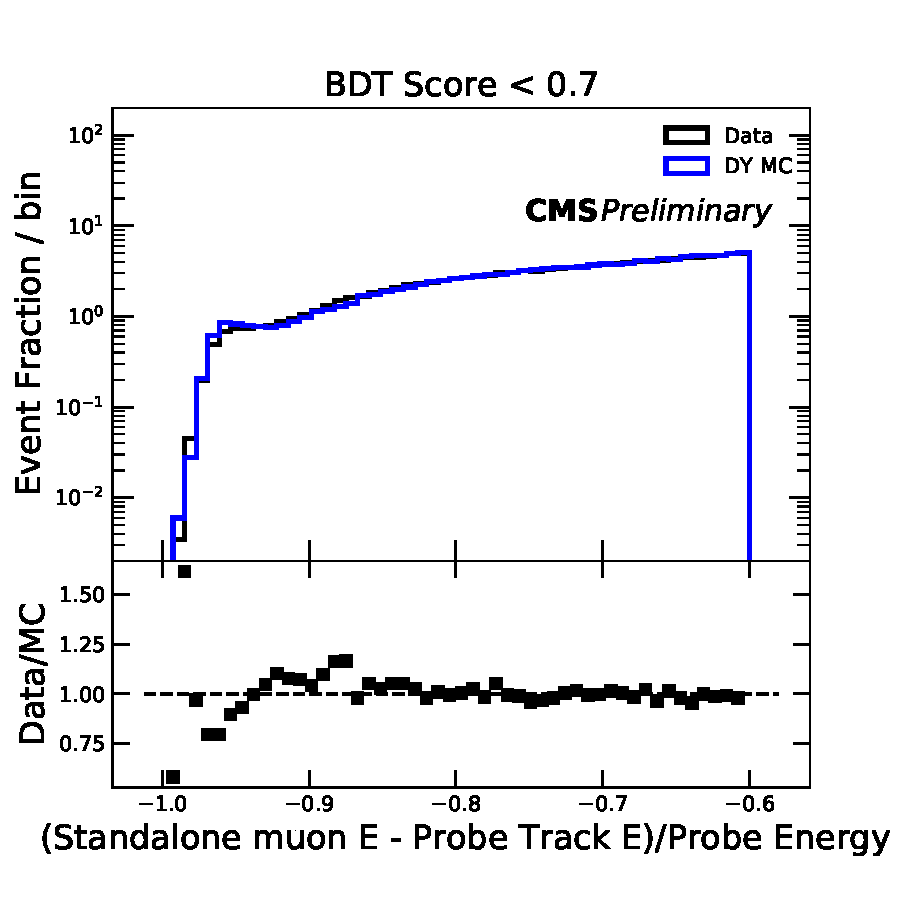
\includegraphics[width=0.45\textwidth]{figures/partialRegionstandaloneDEoverE.pdf}
	\vspace{0.01\textwidth}
	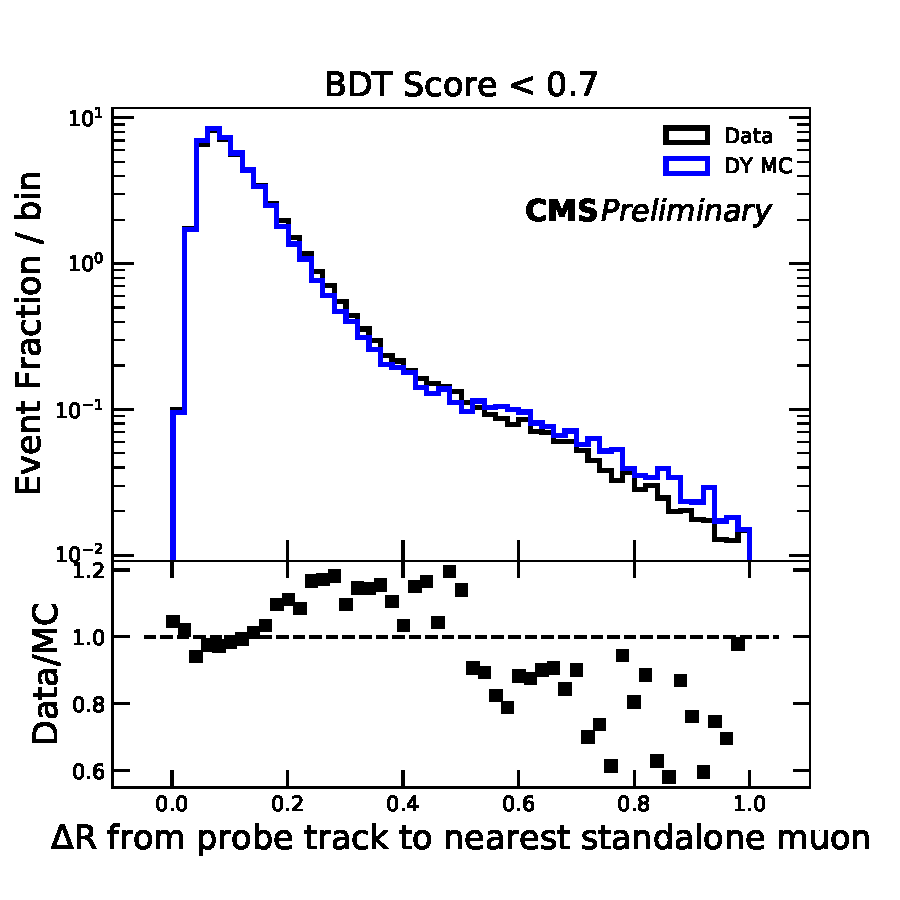
\includegraphics[width=0.45\textwidth]{figures/partialRegionstaDR.pdf}
	\hspace{0.01\textwidth}
	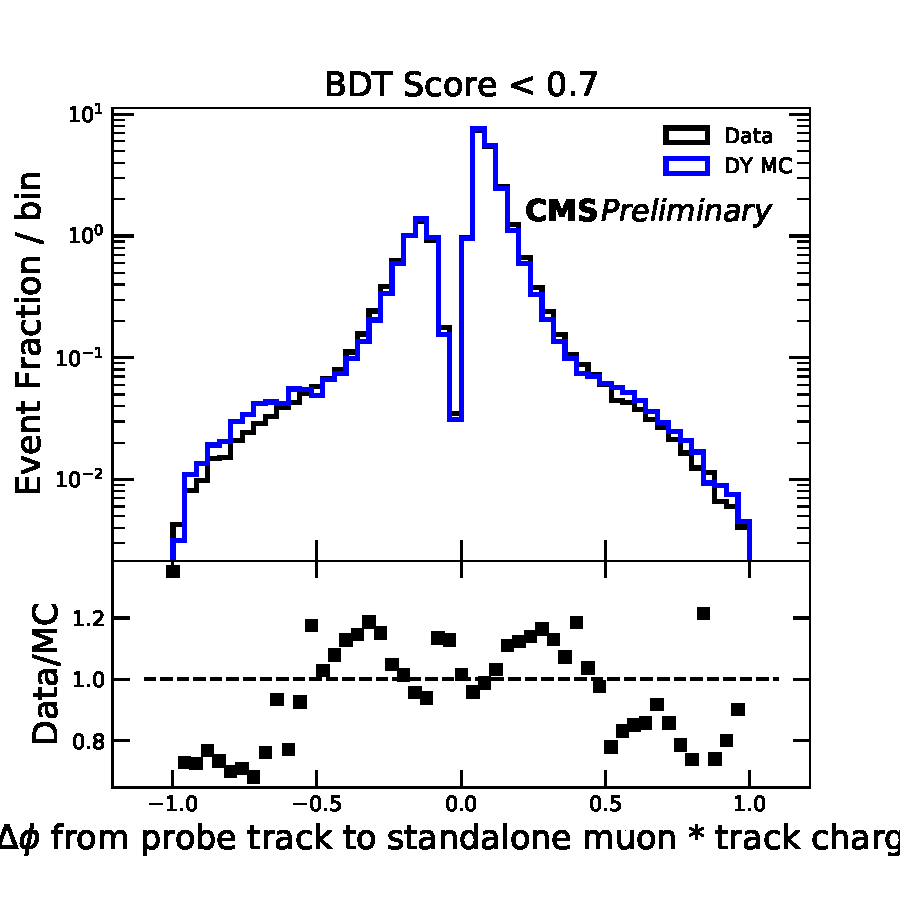
\includegraphics[width=0.45\textwidth]{figures/partialRegionstaPhi.pdf} 
        \caption[Low-Score Event Validation After Correction]{The input features which originally showed significant differences between data and DY simulation in the low BDT score control region after removing events with large angular differences between the first and later CSC stations.}
\end{figure}

The resulting BDT score for DY MC and low-score data events is shown in \Cref{fig:BDTlowvalid}.
Good agreement is in the BDT score, as well as the individual input features.

\begin{figure}[htbp]
	\label{fig:BDTlowvalid}
	\centering
	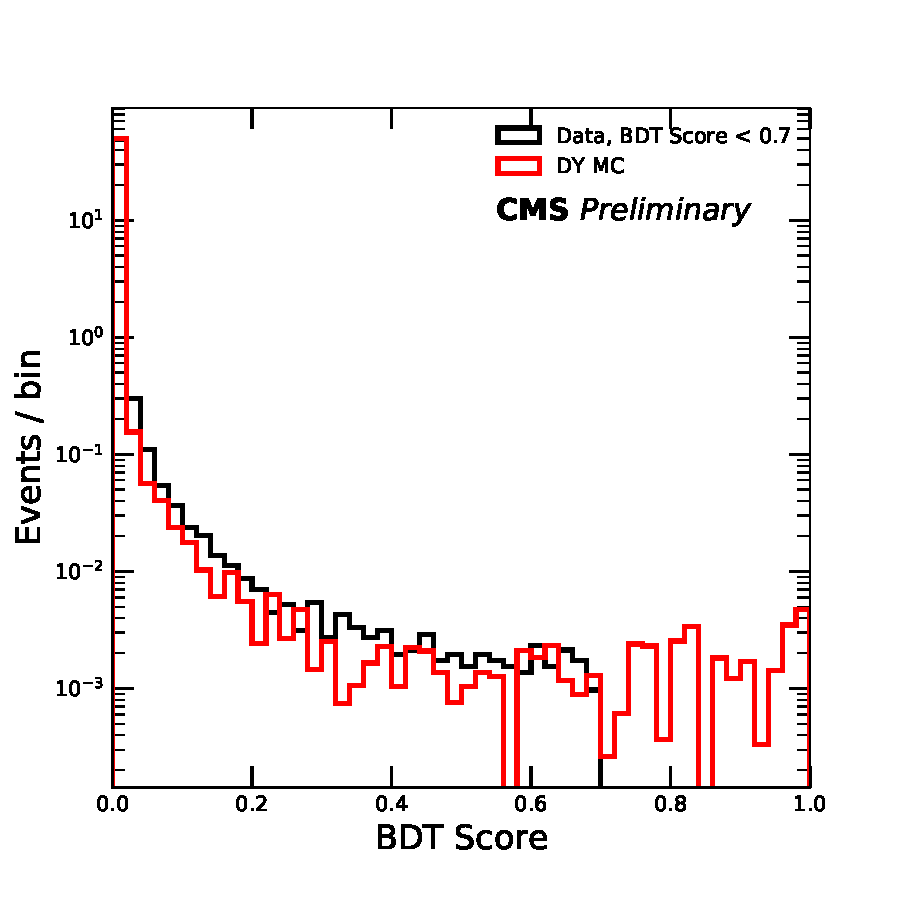
\includegraphics[width=0.5\textwidth]{figures/partialBDTScore.pdf}
        \caption[Low BDT Score Validation]{The distribution of BDT output scores for all DY MC events and for data events with BDT scores less than 0.7.}
\end{figure}

